%This is the first chapter of the dissertation

%The following command starts your chapter. If you want different titles used in your ToC and at the top of the page throughout the chapter, you can specify those values here. Since Columbia doesn't want extra information in the headers and footers, the "Top of Page Title" value won't actually appear.

\chapter[Object Reconstruction][Top of Page Title]{Object Reconstruction}

This chapter describes the reconstruction algorithms used within ATLAS.
We will make the distinction between the ``primitive'' objects which are reconstructed from the detector signals from the ``composite'' physics objects we use in measurements and searches for new physics.

\section{Primitive Object Reconstruction}

The primitive objects reconstructed by ATLAS are \textit{tracks} and (calorimeter) \textit{clusters}.
These are reconstructed directly from tracking hits and calorimeter energy deposits into cells.
Tracks can be further divided into inner detector and muon spectrometer tracks.
Calorimeter clusters can be divided into sliding-window clusters and topological clusters (topoclusters).
% \footnotemark
% \footnotetext{Strictly speaking, sliding-window and topological clustering are the names of the algorithms, and thus one could speak of topological electromagnetic clusters or hadronic sliding-window clusters.
% In ATLAS, sliding-window is almost exclusively used to reconstruct electromagnetic objects and topological clustering is almost exclusively used for hadronic clustering, so to avoid confusion we will use this terminology here.
% These choices are entirely based on optimizing the object reconstruction efficiency relative to the fake rate.
% }
\subsection{Inner Detector Tracks}\label{sec:id_tracks}

Inner detector tracks are reconstructed from hits in the inner detector \cite{ATLAS-CONF-2012-042,ATL-PHYS-PUB-2015-051}
These hits indicate that a charged particle has passed through the detector material.
Due to the 2 T solenoid in the inner detector, the hits associated with any individual particle will be curved.
The amount of curvature determines the momentum of the particle.
In any given event, there is upwards of 10$^4$ hits, making it impossible to do any sort of combinatorics to reconstruct tracks.
There are two algorithms used by ATLAS track reconstruction, known as \textit{inside-out} and \textit{outside-in}.

ATLAS first employs the inside-out algorithm.
One assumes the track begins at the interaction point.
Moving out from the interaction point, one creates track seeds.
Track seeds are proto-tracks constructed from three hits.
These hits can be distributed as three pixel hits, two pixel hits and one SCT hit, or three SCT hits.
One extrapolates the track and uses a combinatorial Kalman filter\cite{ATLAS-CONF-2012-042}, which adds the rest of the pixel and SCT hits to the seeds.
This is done seed by seed, so it avoids the combinatorial complexity involved with checking all hits with all seeds.
At this point, the algorithm applies an additional filter to avoid ambiguities from nearby tracks.
The TRT hits are added to the seeds using the same method.
After this procedure, all hits are associated to a track.

The next step is to figure out the correct kinematics of the track.
This is done by applying a fitting algorithm which outputs the best-fit track parameters by minimizing the track distance from hits, weighted by each hit's resolution.
These parameters are $(d_0, z_0, \eta, \phi, q/p)$ where $d_0$ ($z_0$) is the transverse (longitudinal) impact parameter and $q/p$ is the charge over the track momenta.
This set of parameters uniquely defines the measurement of the trajectory of the charged particle associated to the track.
An illustration of a track with these parameters is shown in Fig.\ref{fig:track_schematic}.

\begin{figure}
\caption{The parameters associated to a track.}
\label{fig:track_schematic}
\includegraphics[width=.9\linewidth]{track_schematic}
\end{figure}

The other track reconstruction algorithm is the outside-in algorithm.
As the name implies, we start from the outside of the inner detector, in the TRT, and extend the tracks in toward the interaction point.
One begins by seeding from TRT hits, and extending the track back towards the center of the detector.
The same fitting procedure is used as in the inside-out algorithm to find the optimal track parameters.
This algorithm is particularly important for finding tracks which originate from interactions with the detector material, especially the SCT.
For tracks from primary vertices, this often finds the same tracks as the inside-out algorithm, providing an important check on the consistency of the tracking procedure.

In the high luminosity environment of the LHC, even the tracks reconstructed from precision detectors such as those of ATLAS inner detector can sometimes lead to fake tracks from simple combinatoric chance.
Several quality checks are imposed after track fitting which reduce this background.
Seven silicon (pixel + SCT) hits are required for all tracks.
No more than two \textit{holes} are allowed in the pixel detector.
Holes are expected measurements from the track that are missing in the pixel detector.
Finally, tracks with poor fit quality, as measured by $\chi^2/ndf$, are also rejected.
Due to the high quality of the silicon measurements in the pixel detector and SCT, these requirements give good track reconstruction efficiency, as seen in Fig.\ref{fig:track_eff} for simulated events\cite{Hamano:1489674}.
\begin{figure}
\caption{Track reconstruction efficiency as a function of track \pt and $\eta$.
The efficiency is defined as the number of reconstructed tracks divided by the number of generate charged particles.} \label{fig:track_eff}
\subfloat[Track reconstruction as a function of \pt.]   {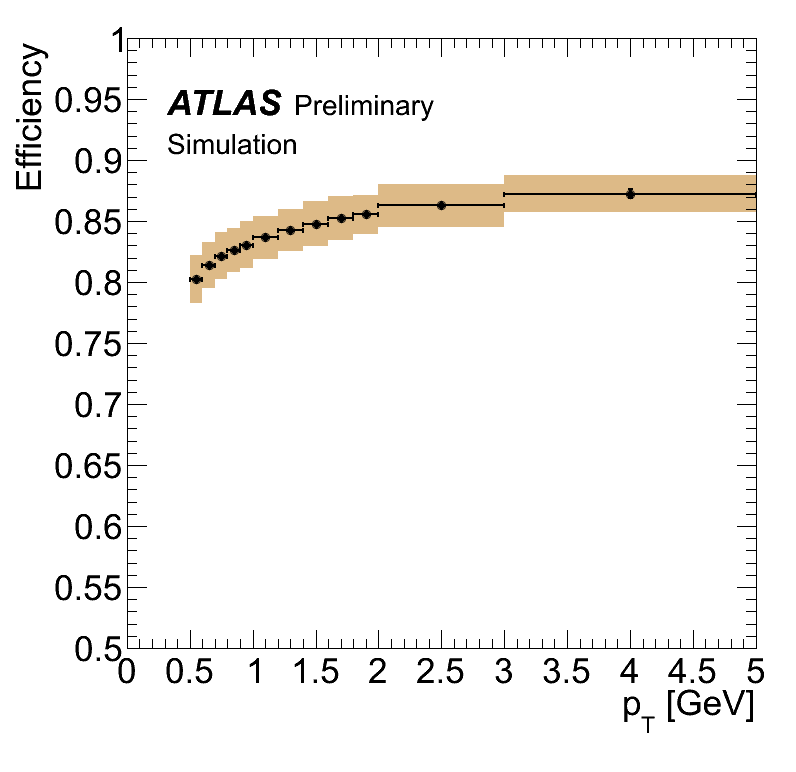
\includegraphics[width=.45\linewidth]{track_eff_pt}}
\subfloat[Track reconstruction as a function of $\eta$.]{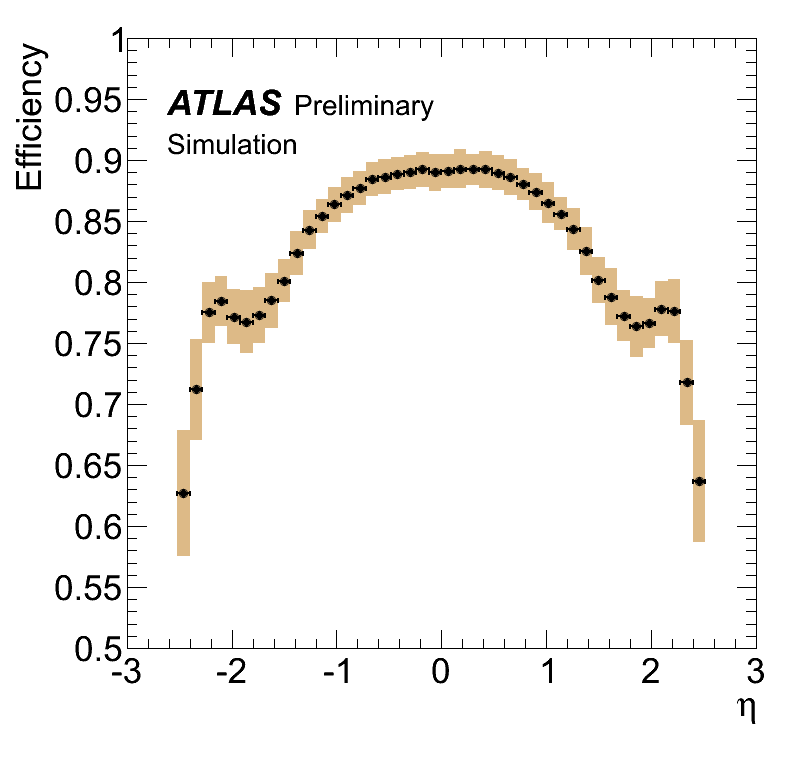
\includegraphics[width=.45\linewidth]{track_eff_eta}} \\
\end{figure}

\subsection{Sliding-window clusters}\label{sec:sliding_window_cluster}

The sliding-window algorithm is a way to combine calorimeter cells into composite objects (clusters) to be used as inputs for other algorithms\cite{PERF-2013-03}.
Sliding-window clusters are the primary inputs to electron and photon reconstruction, as described below.
The electromagnetic calorimeter has high granularity, with a cell size of $(\eta, \phi) = (.025, .025)$ in the coarsest second layer throughout most of the calorimeter.
The ``window'' consists of 3 by 5 cells in the $(\eta, \phi)$ space.
All layers are added on this same 2D space.
One translates this window over the space and seeds a cluster whenever the energy sum of the cells is maximized.
If the seed energy is greater than 2.5 \GeV, this seed is called a sliding-window cluster.
This choice was motivated to optimize the reconstruction efficiency of proto-electrons and proto-photons while rejecting fakes from electronic noise and additional particles from pileup vertices.

\subsection{Topological clusters}\label{sec:topoclusters}

Topoclusters are the output of the algorithm used within ATLAS to combine hadronic and electromagnetic calorimeter cells in a way which extracts signal from a background of significant electronic noise\cite{PERF-2014-07}.
They are the primary input to the algorithms which reconstruct jets.

Topological clusters are reconstructed from calorimeter cells in the following way.
First, one maps all cells onto a single $\eta-\phi$ plane so one can speak of \textit{neighboring} cells.
Two cells are considered neighboring if they are in the same layer and directly adjacent, or if they are in adjacent layers and overlap in $\eta-\phi$ space.
The \textit{significance} $\xi_{\text{cell}}$ of a cell during a given event is

\begin{equation}
\calosig = \frac{E_{\text{cell}}}{\sigma_{\text{noise,cell}}}
\end{equation}

where $\sigma_{\text{noise,cell}}$ is measured for each cell in ATLAS and $E_{\text{cell}}$ measures the current energy level of the cell.
One thinks of this as the measurement of the energy \textit{over threshold} for the cell.

Topocluster \textit{seeds} are defined as calorimeter cells which have a significance $\calosig > 4 $.
These are the inputs to the algorithm.
One iteratively tests all cells adjacent to these seeds for $\calosig > 2$.
Each cells passing this selection is then added to the topocluster, and the procedure is repeated.
When the algorithm reaches the point where there are no additional adjacent cells with $\calosig > 2$, every positive-energy cell adjacent to the current proto-cluster is added.
The collection of summed cells is a topocluster.
An example of this procedure for a simulation dijet event is shown in Fig.\ref{fig:topocluster}.
\begin{figure}
\caption{Example of topoclustering on a simulated dijet event.} \label{fig:topocluster}
\subfloat[All cells with $\calosig > 4$.]{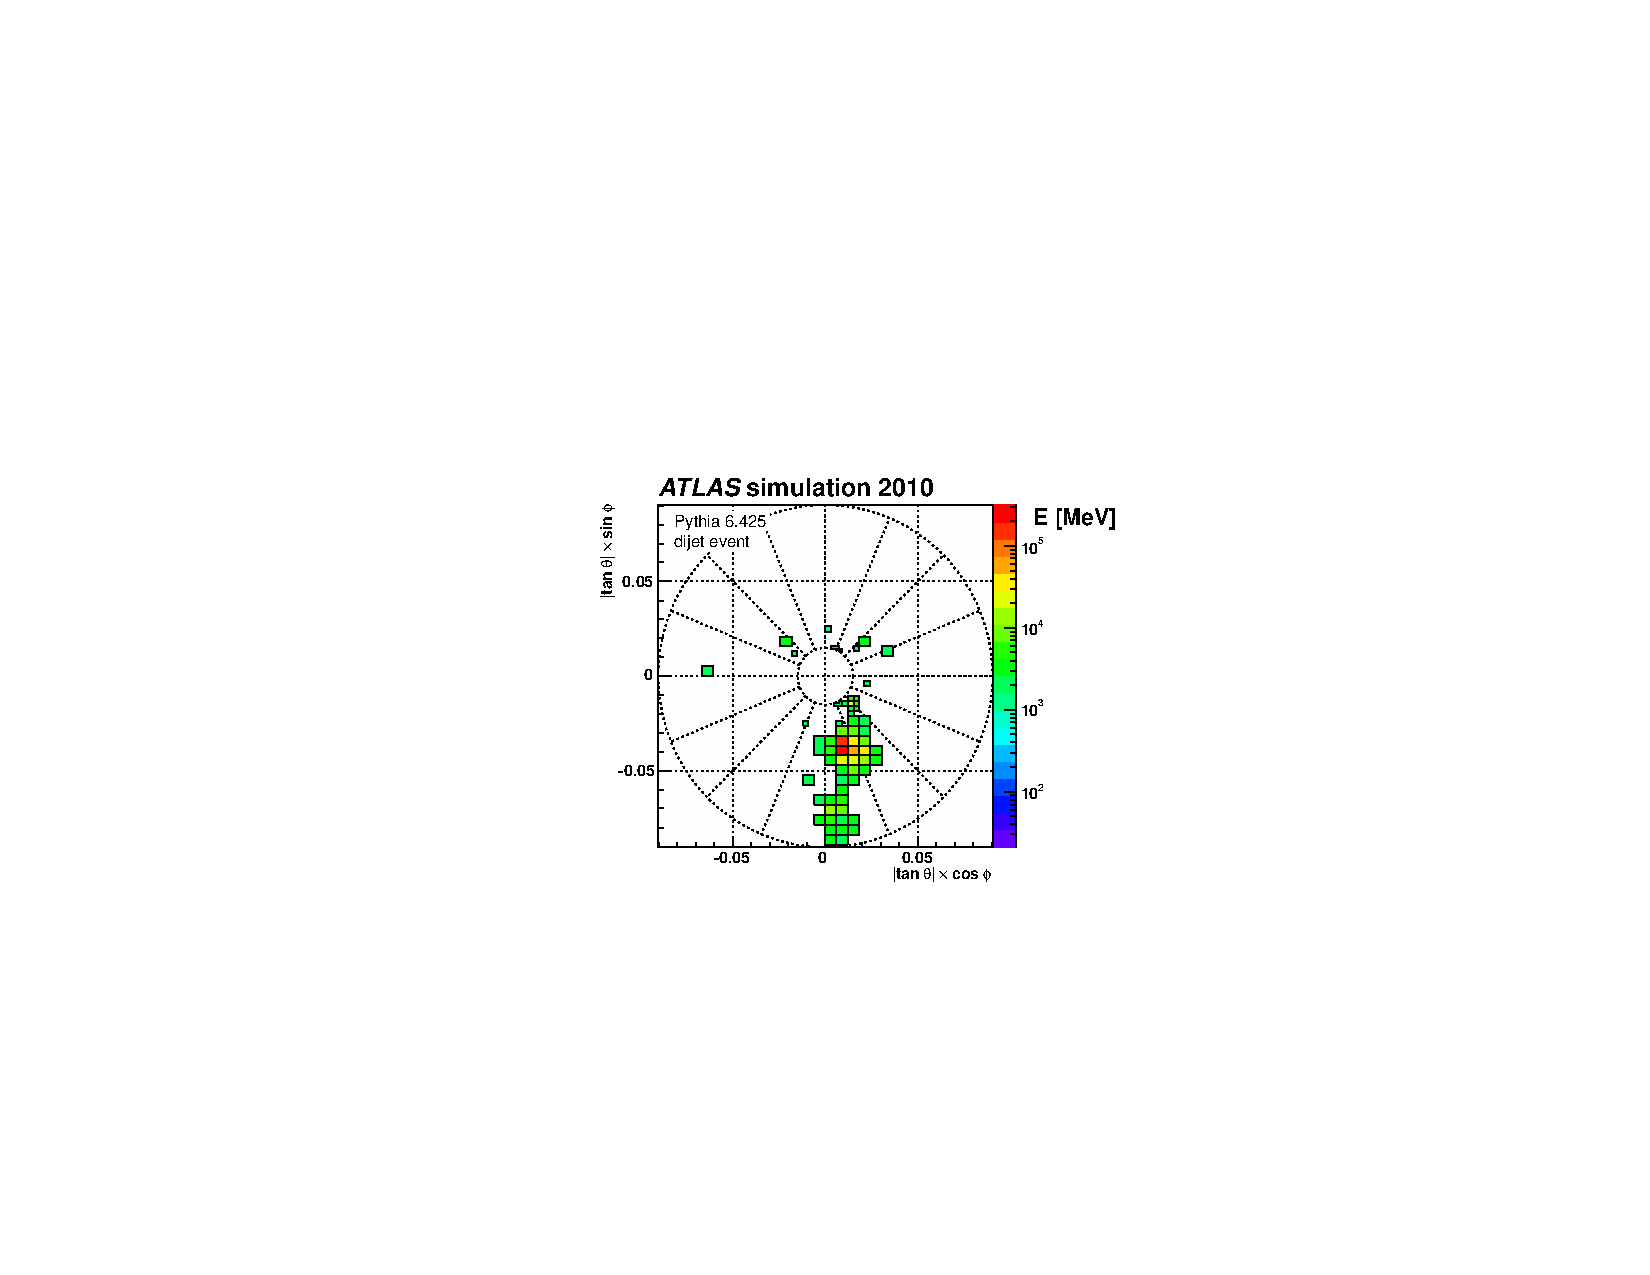
\includegraphics[width=.45\linewidth]{topoclustering_sig4.pdf}}
\subfloat[All cells with $\calosig > 2$.]{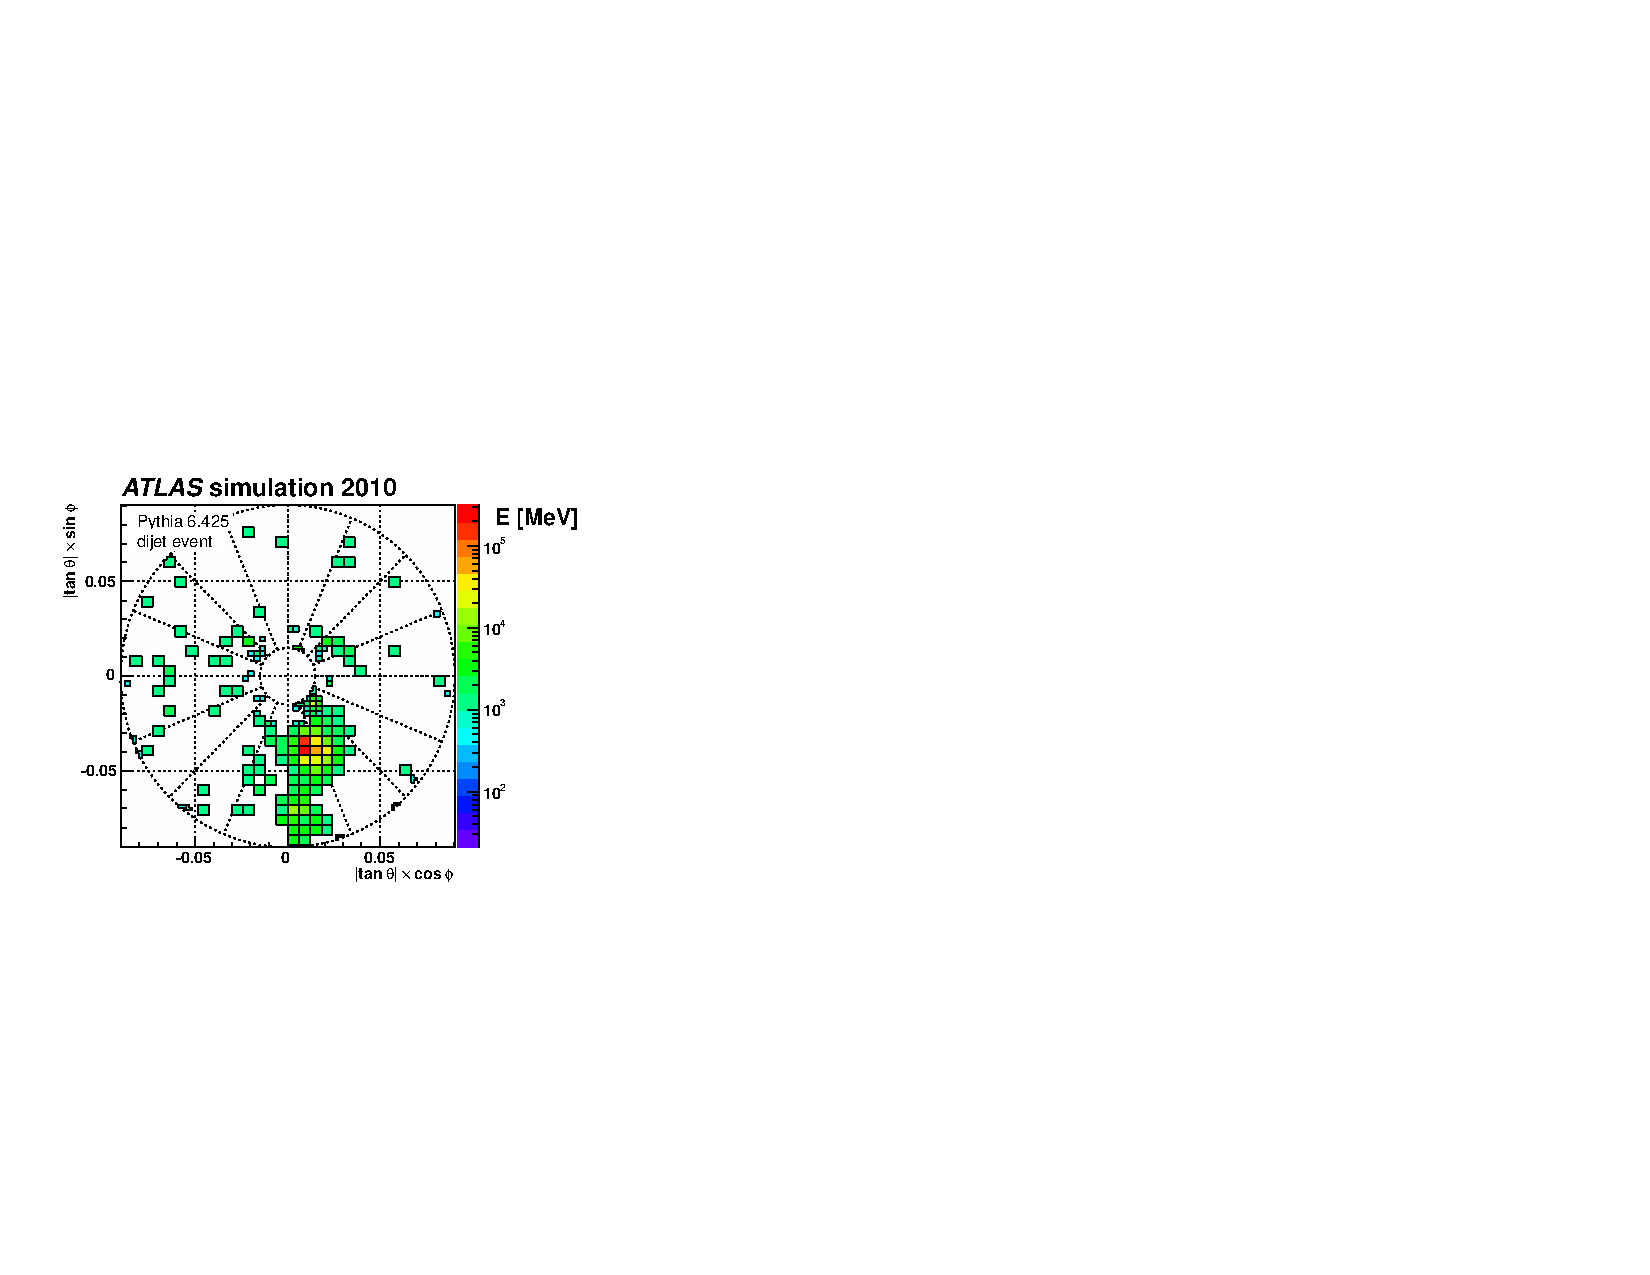
\includegraphics[width=.45\linewidth]{topoclustering_sig2.pdf}} \\
\subfloat[All clustered cells.]{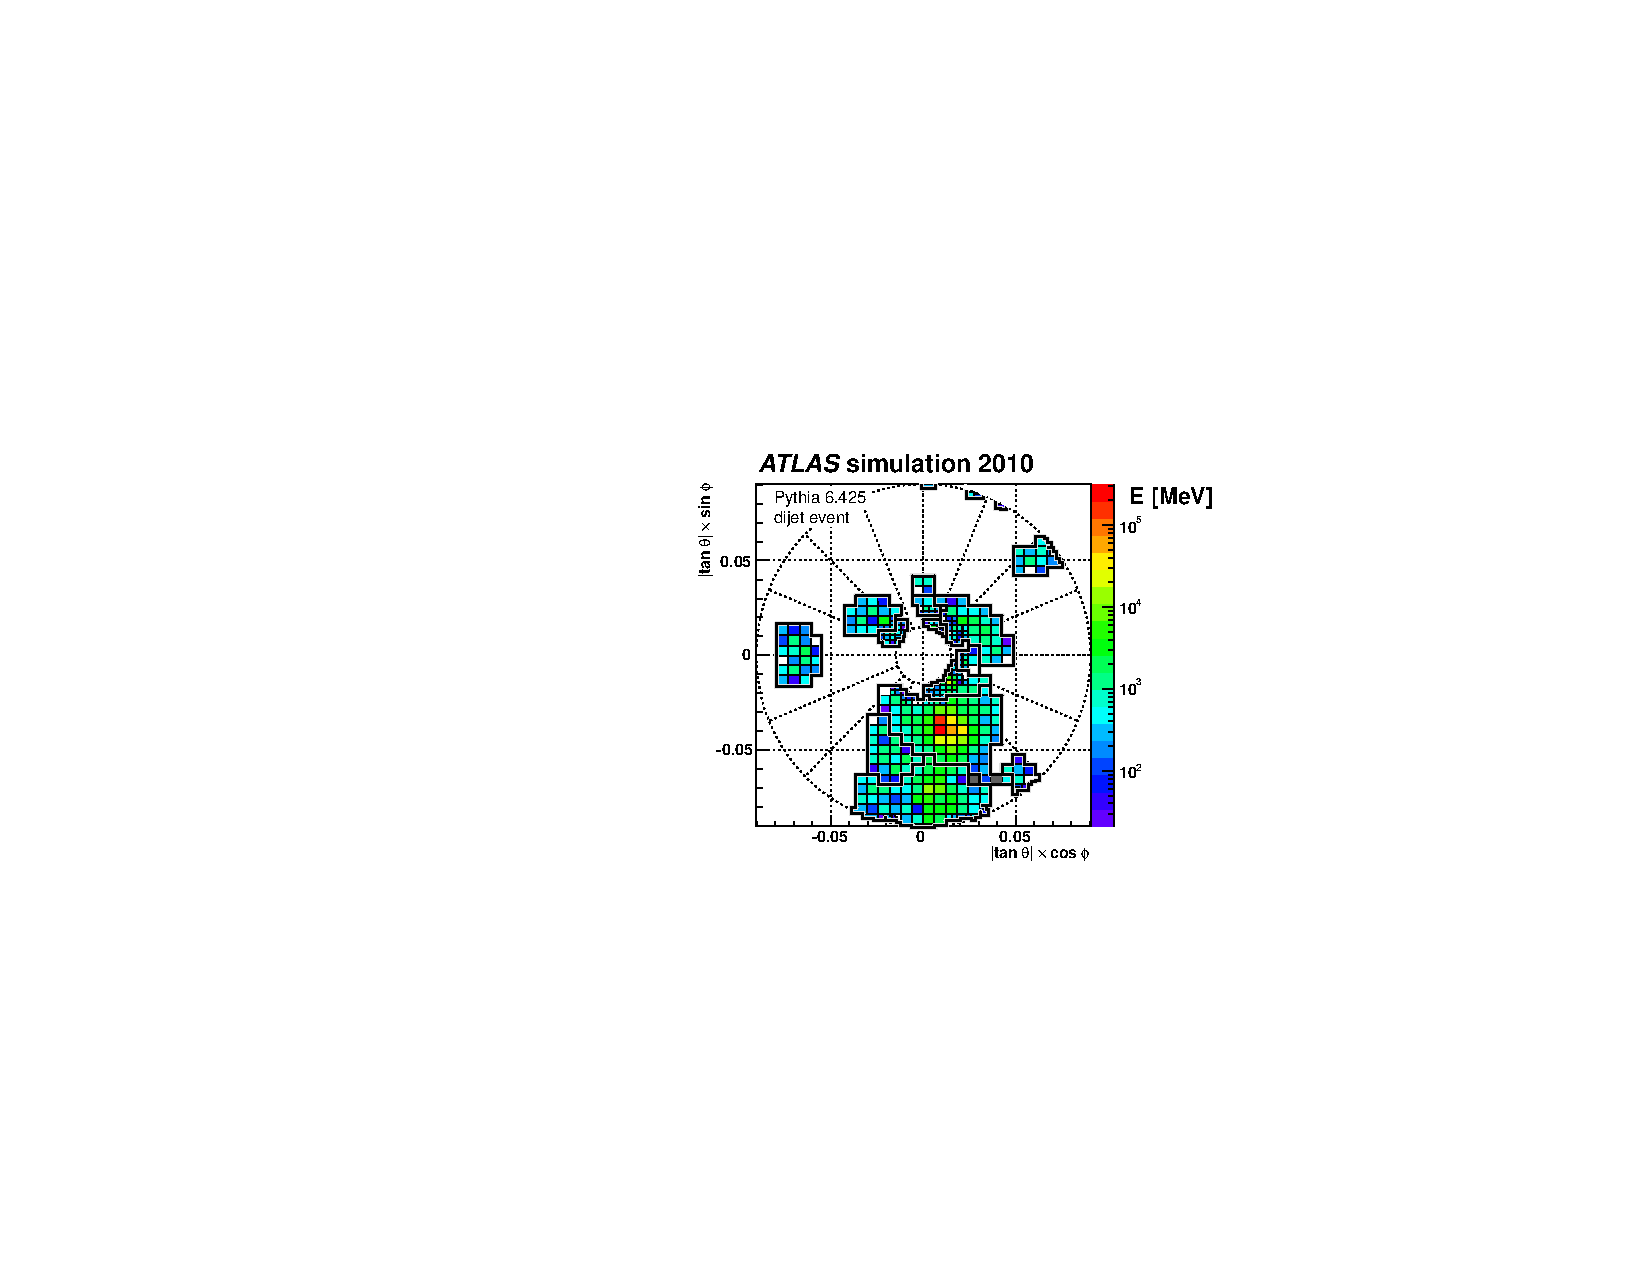
\includegraphics[width=.9\linewidth]{topoclustering_sig0.pdf}}
\end{figure}

There are two calibrations used for clusters\cite{PERF-2011-04}.
These are known as the electromagnetic (EM) scale and the local cluster weighting (LCW) scale.
The EM scale is the energy read directly out of the calorimeters as described.
This scale is appropriate for electromagnetic processes.
The LCW scale applies additional scaling to the clusters based on the shower development.
The cluster energy can be corrected for calorimeter non-compensation and the differences in the hadronic and electromagnetic calorimeters' responses.
This scale provides additional corrections that improve the accuracy of hadronic energy measurements.
This thesis only uses the EM scale corrections.
LCW scaling requires additional measurements that only became available with additional data.
Due to the jet calibration procedure that we will describe below, it is also a relatively complicated procedure to rederive the ``correct'' jet energy.

\subsection{Muon Spectrometer Tracks}\label{sec:ms_tracks}

Muon spectrometer tracks are fit using the same algorithms as the ID tracks, but different subdetectors.
The tracks are seeded by hits in the MDTs or CSCs.
After seeding in the MDTs and CSCs, the hits from all subsystems are refit as the final MS track.
These tracks are used as inputs to the muon reconstruction, as we will see below.

\section{Physics Object Reconstruction and Quality Identification}

There are essentially six objects used in ATLAS searches for new physics: electrons, photons, muons, $\tau$-jets, jets, and \met.
The reconstruction of these objects is described here.
In this thesis, $\tau$ lepton jets are not treated differently from other hadronic jets, and we will not consider their reconstruction algorithms.
A very convenient summary plot is shown in Fig.\ref{fig:atlas_interactions}.
\begin{figure}
\caption{The interactions of particles with the ATLAS detector.
Solid lines indicate the particle is interacting with the detector, while dashed lines are shown where the particle does not interact.} \label{fig:atlas_interactions}
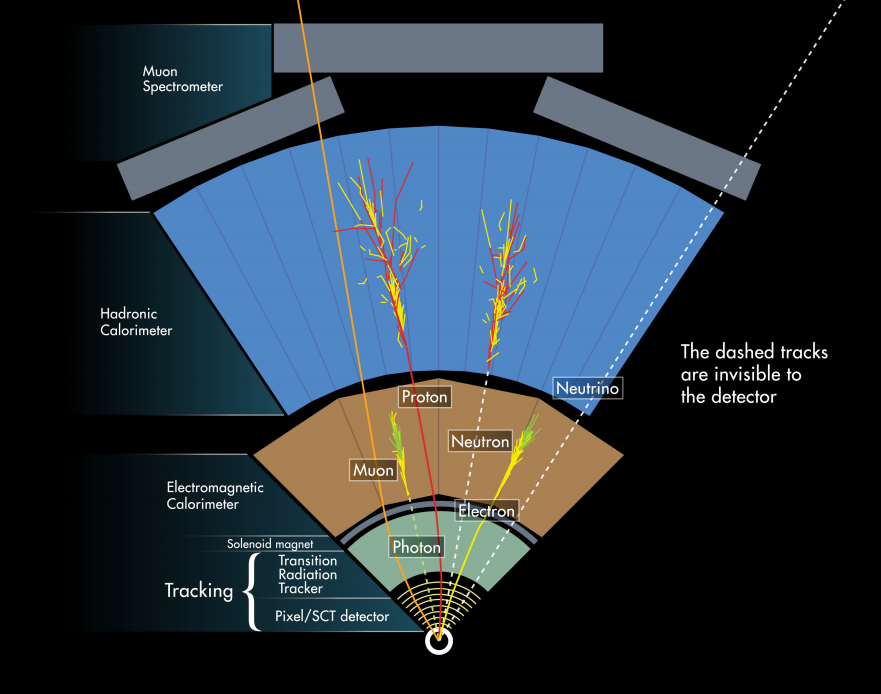
\includegraphics[width=.9\linewidth]{atlas_particle_interactions}
\end{figure}

One often wishes to understand ``how certain'' we are that a particular object is truly the underlying physics object.
In ATLAS, we often generically consider, in order, \textit{very loose}, \textit{loose}, \textit{medium}, and \textit{tight} objects\footnotemark.
\footnotetext{
These are not all used for all objects, but it's conceptally useful to think of these different categories.
}
These are ordered in terms of decreasing object efficiency, or equivalently, decreasing numbers of fake objects.
We will also describe briefly the classification of objects into these categories.

In this thesis, since we present a search for new physics in a zero lepton final state, we will provide additional details about jet and \met reconstruction.
% \subsection{Vertices}

% Vertex reconstruction is an important first step in the reconstruction of ATLAS events\cite{ATL-INDET-PUB-2009-001}.
% If two tracks from charged particles point at the same place inside the detector, we can associate these tracks to that point, which we then call a vertex.
% Generally, we speak of primary vertices associated
% \begin{figure}
% \caption{Depiction of different vertices reconstruct by ATLAS.
% Each ATLAS event has the primary vertex, b-physics vertices, and pileup vertices.} \label{fig:topocluster}
% 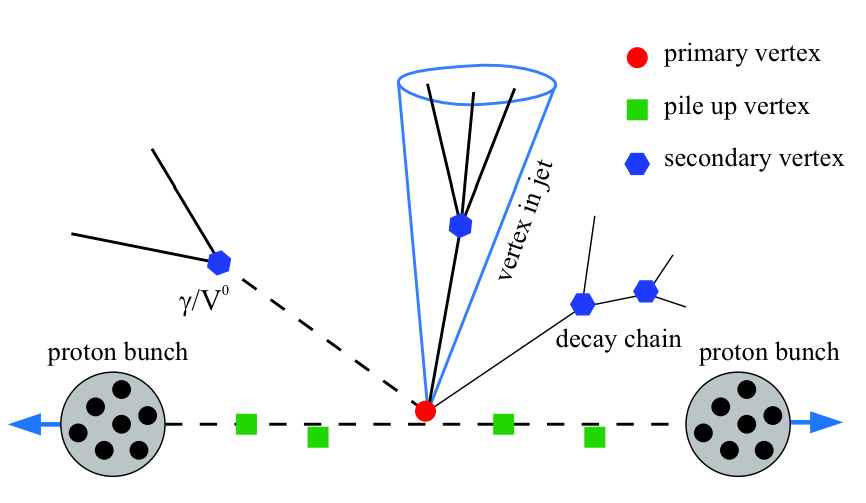
\includegraphics[width=.45\linewdith]{vertex_reconstruction} \\
% \end{figure}

\subsection{Electrons and Photons}

\subsubsection{Reconstruction}
The reconstruction of electrons and photons (often for brevity called ``electromagnetic objects'') is very similar \cite{Aaboud:2016yuq,PERF-2013-05,PERF-2013-03}.
This is because the reconstruction begins with the energy deposit in the calorimeter in the form of an electromagnetic shower.
For any incoming $e/\gamma$, this induces many more electrons and photons in the shower.
The measurement in the calorimeter is similar for these two objects.

One begins the reconstruction of electromagnetic objects from the sliding-window clusters reconstructed from the EM calorimeter.
These $E > 2.5 \GeV$ clusters the the primary seed for electrons and photons.
One then looks for all ID tracks within $\deltaR < 0.3$, where $\deltaR = \sqrt{\Delta\eta^2 + \Delta\phi^2}$.
We ``match'' the track and cluster if they are within $\Delta \phi < 0.2$ in the direction of track curvature, or $\Delta \phi < 0.05$ in the direction opposite the track curvature.
Those track-cluster seeds with tracks pointing to the primary vertex are reconstructed as electrons.

For photons, we have two options to consider, known as \textit{converted} and \textit{unconverted} photons.
Due to the high energy of the LHC collisions, typical photons have energy $ >\order 1 \GeV$.
At this scale, photons interact almost exclusively via pair-production in the presence of the detector material, as shown in Fig.\ref{fig:photon_pair_production} \cite{Agashe:2014kda}.
If the track-cluster seed has a track which does not point at the primary vertex, we reconstruct this object as a converted photon.
This happens since the photon travels a distance before decay into two electrons, and see the tracks coming from this secondary vertex.
Those clusters which do not have any associated tracks are then reconstruced as an unconverted photon.
\begin{figure}
\caption{Photon total cross sections as a function of energy in carbon and lead, showing the contributions of different processes\cite{Agashe:2014kda}.} \label{fig:photon_pair_production}
\includegraphics[width=.75\linewidth]{sigma_both_06}
\end{figure}

The final step in electromagnetic object reconstruction is the final energy value assigned to these objects.
This process is different between electrons and photons due to their differing signatures in the EM calorimeter.
In the barrel, electrons energies are assigned as the sum of the 3 clusters in $\eta$ and 7 clusters in $\phi$ to account for the electron curving in the $\phi$ direction.
Barrel photons are assigned the energy sum of $(3,5)$ clusters in $(\eta, \phi)$ space.
In the endcap, the effect of the magnetic field on the electrons is smaller, and there is a coarser granularity.
Both objects sum the $(5,5)$ clusters for their final energy value.

\subsubsection{Quality Identification}

Electrons have a number of important backgrounds which can give fakes.
Fake electrons come primarily from secondary vertices in hadron decays or misidentified hadronic jets.
To reduce these backgrounds, quality requirements are imposed on electron candidates.
Loose electrons have requirements imposed on the shower shapes in the electromagnetic calorimeter and on the quality of the associated ID track.
There is also a requirement that there is a small energy deposition in the hadronic calorimeter behind the electron, to avoid jets being misidentified as electrons (low hadronic leakage).
Medium and tight electrons have increasingly stronger requirements on these variables, and additional requirements on the isolation (as measured by $\Delta R$) and matching of the ID track momentum and the calorimeter energy deposit.

Photons are relatively straightforward to measure, since there are few background processes\cite{ATL-PHYS-PUB-2016-015}.
The primary one is pion decays to two photons, which can cause a jet to be misidentified as photon.
Loose photons have requirements on the shower shape and hadronic leakage.
Tight photons have tighter shower shape cuts, especially on the high granularity first layer of the EM calorimeter.
The efficiency for unconverted tight photons as a function of $\pt$ is should in
\begin{figure}
\caption{Unconverted photon efficiency as measured in \cite{ATL-PHYS-PUB-2016-015}.} \label{fig:photon_eff}
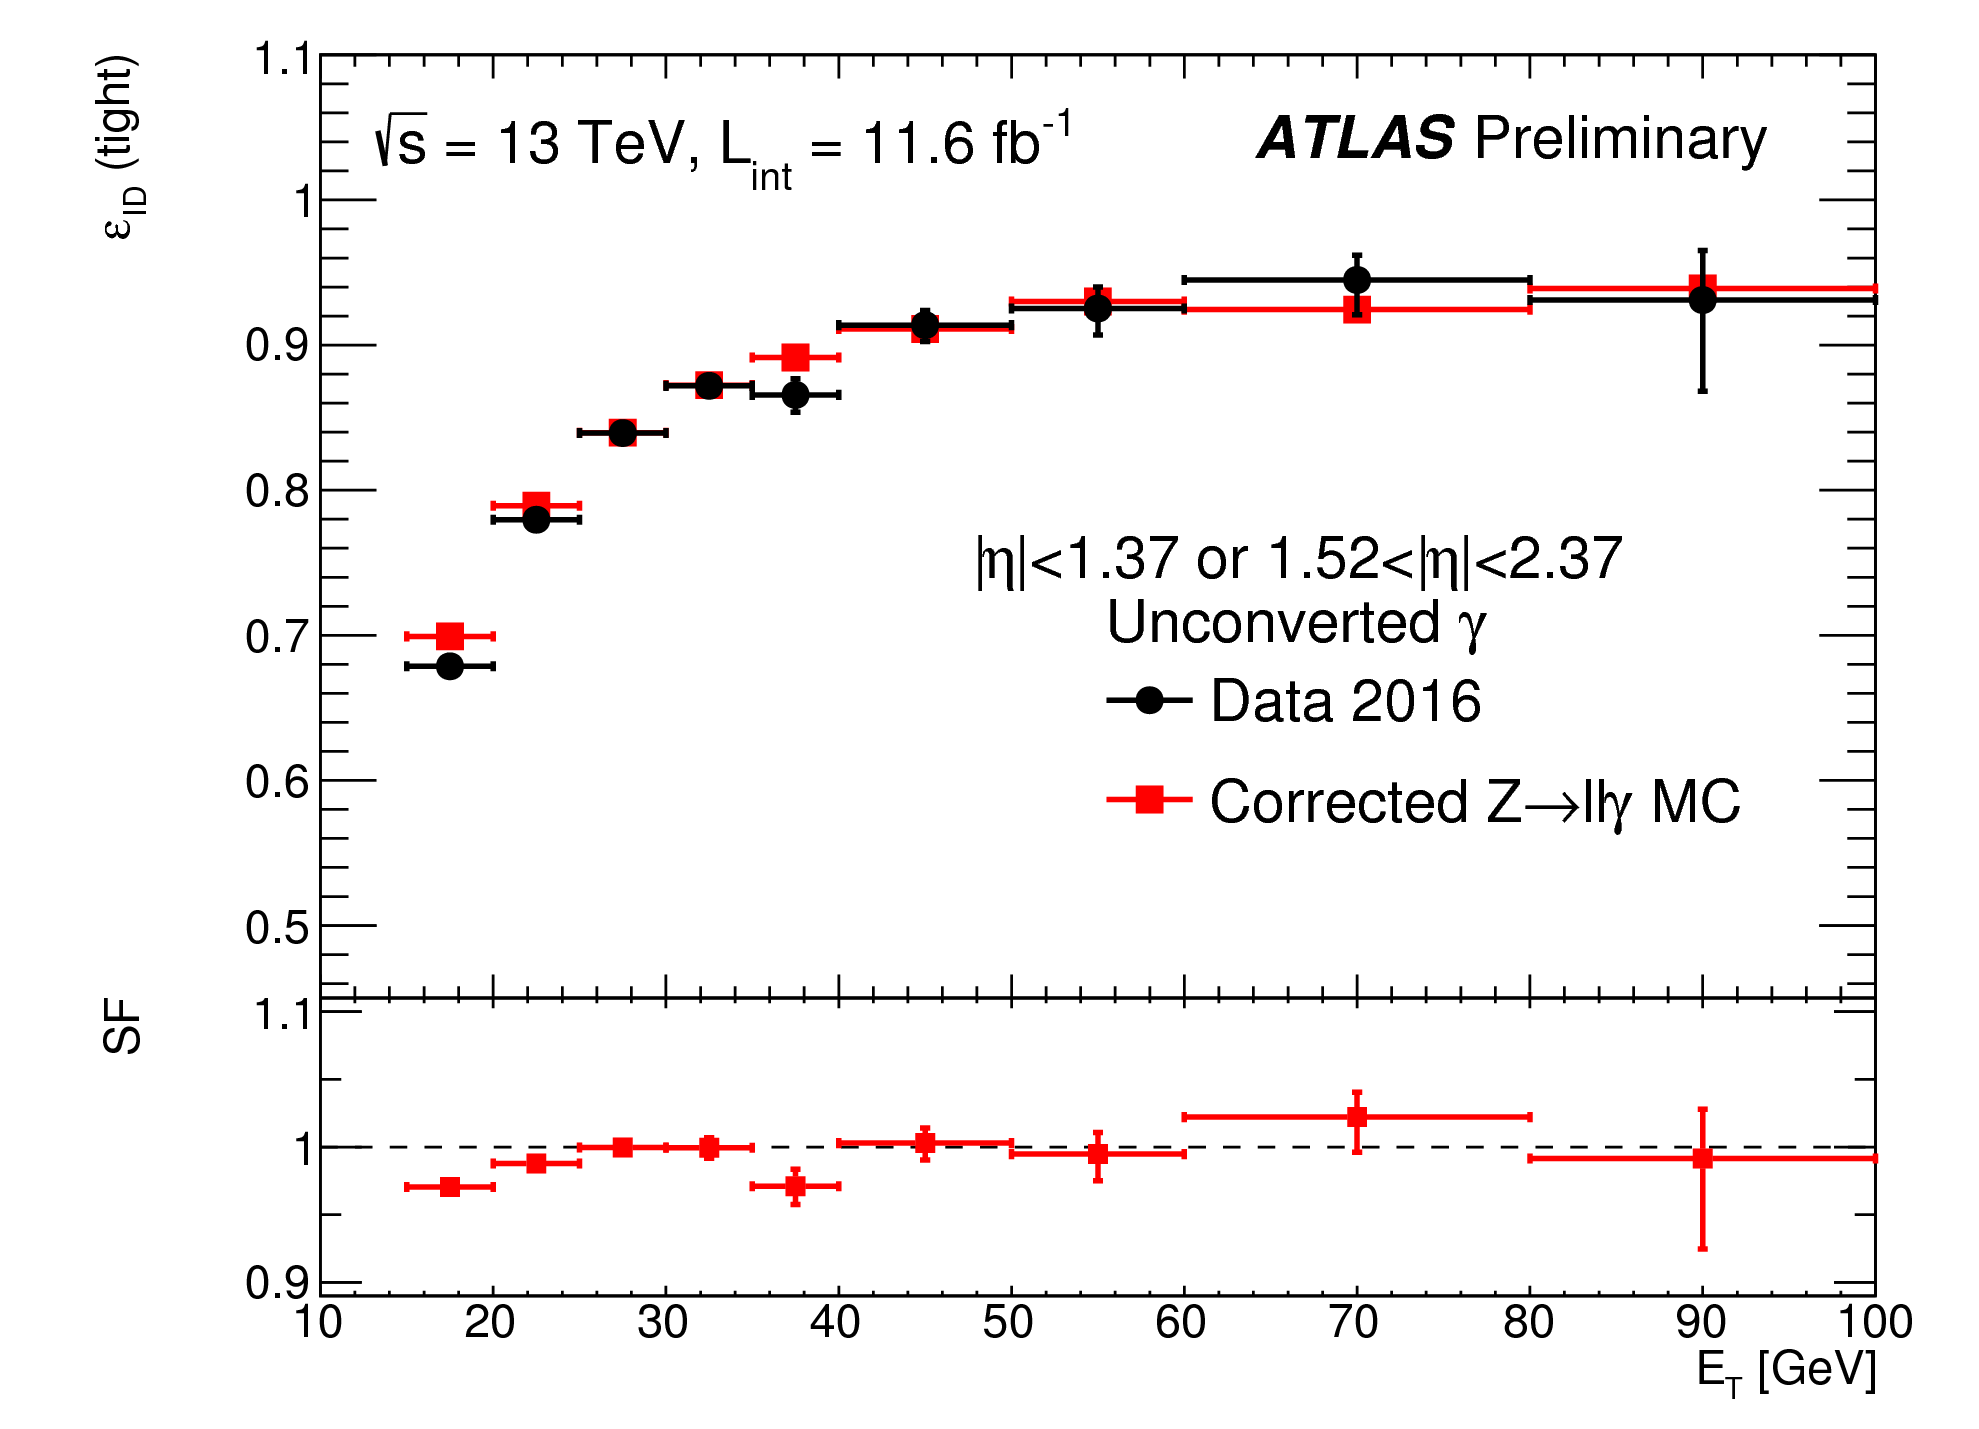
\includegraphics[width=.9\linewidth]{photon_efficiency}
\end{figure}

\subsection{Muons}

\subsubsection{Reconstruction}

Muons are reconstructed using measurements from all levels of the ATLAS detector\cite{PERF-2015-10}.
They leave a ID track, a small, characteristic deposition in the EM calorimeter, and then a track in the muon spectrometer.
The primary reconstruction technique produces a so-called \textit{combined} muon.
``Combined'' means using a combination of the ID and MS tracks to produce the final reconstruced muon kinematics.
This is done by refitting the hits associated to both tracks, and using this refit track for the muon kinematics.
This process produces the best measured muons, although several other worse algorithms are used when the full detector information is missing.
An example is in the region $2.5 < |\eta| < 2.7$ outside the ID acceptance, where MS tracks are used without the corresponding ID tracks.

\subsubsection{Quality Identification}

Several additional criteria are used to assure muon measurements are free of significant background contributions, especially from pion and kaon decays to muons.
Muons produced via these decay processes are often characterized by a ``kink''.
Candidate muons with a poor fit quality, characterized by $\chi^2/\text{n.d.f.}$, are thus rejected.
Additionally, the absolute difference in momentum measurements between the ID and MS provide another handle, since the other decay products from hadron decays carry away some amount of the initial hadron momentum.
This is measured by
\begin{equation}
\rho' = \frac{|\pt^{\text{ID}} - \pt^{\text{MS}} |}{\pt^{\text{Combined}}}.
\end{equation}
Additionally, there is a requirement on the $q/p$ significance, defined as
\begin{equation}\label{eq:muon_sig}
S_{q/p} = \frac{|(q/p)^{\text{ID}} - (q/p)^{\text{MS}} |}{\sqrt{\sigma_{\text{ID}}^2 + \sigma_{\text{MS}}^2  }}.
\end{equation}
The $\sigma_{\text{ID,MS}}$ in the denominator of Eq.\ref{eq:muon_sig} are the uncertainties on the corresponding quantity from the numerator.
Finally, cuts are placed on the number of hits in the various detector elements.

Subsequently tighter cuts on these variables allow one to define the different muon identification criteria.
Loose muons have the highest reconstruction efficiency, but the highest number of fake muons, since there are no requirements on the number of subdetector hits and the loosest requirements on the suite of quality variables.
Medium muons consist of Loose muons with tighter cuts on the quality variables.
They also require more than three MDT hits in at least two MDT layers.
These are the default used by ATLAS analyses.
Tight muons have stronger cuts than those of the medium selection, and reducing the reconstruction efficiency.
The reconstruction efficiency as a function of \pt can be seen for Medium muons in Fig.\ref{fig:muon_eff}.

\begin{figure}
\caption{Medium muon efficiency as measured in \cite{PERF-2015-10}.} \label{fig:muon_eff}
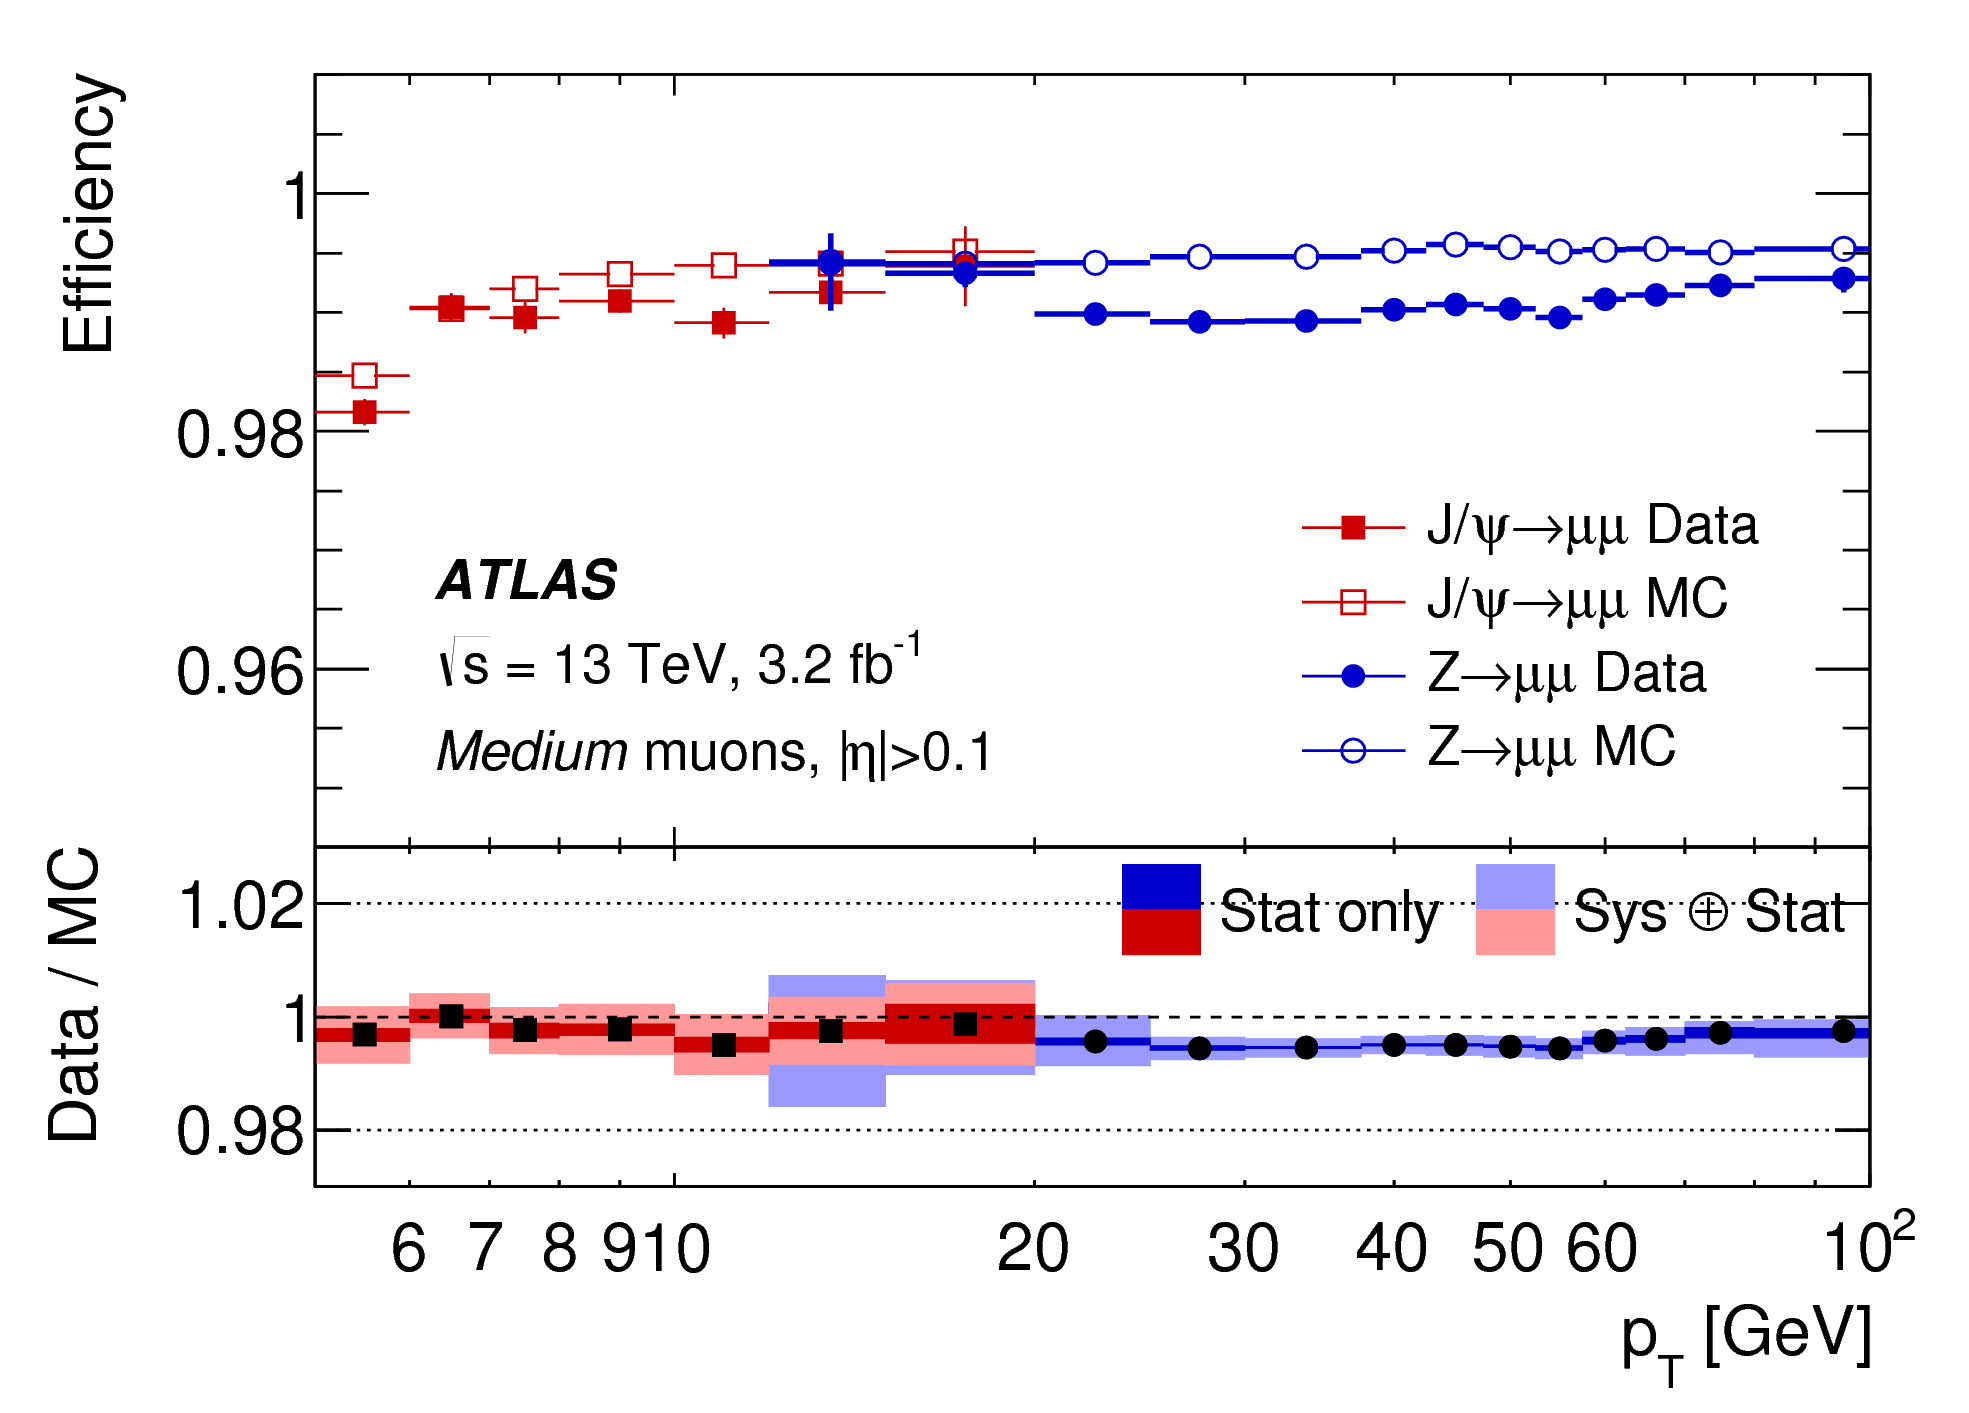
\includegraphics[width=.9\linewidth]{muon_efficiency}
\end{figure}

\subsection{Jets}

Jets are composite objects corresponding to many physical particles \cite{Agashe:2014kda,PERF-2011-03,PERF-2012-01}
This is a striking difference from the earlier particles.
Fortunately, we normally (and in this thesis) care about the original particle produced in primary collision.
In the SM, this corresponds to quarks and gluons.
Due to the hadronization process, free quarks and gluons spontaneously hadronize and produce a hadronic shower, which we call a jet.
These showers can be measured by the EM and hadronic calorimeters, and the charged portions can be measured in the ID.
The first question is how to combine these measurements into a composite object representing the underlying physical parton.
This is done via jet algorithms.

\subsection{Jet Algorithms}

It might seem straightforward to combine the underlying physical particles into a jet.
There are three important characteristics required for any jet reconstruction algorithm to be used by ATLAS.
\begin{itemize}
\item Collinear safety - if any particle with four-vector $p$ is replaced by two particles of $p_1, p_2$ with $p = p_1 + p_2$, the subsequent jet should not change
\item Radiative (infrared) safety - if any particle with four-vector $p$ radiates a particle of energy $\alpha \rightarrow 0$, the subsequent jet should not change
\item Fast - the jet algorithm should be ``fast enough'' to be useable by ATLAS computing resources
\end{itemize}
The first two requirements can be seen in terms of requirements on soft gluon emission.
Since partons emit arbitrarily soft gluons freely, one should expect the algorithms to not be affected by this emission.
The final requirement is of course a practical limitation.

The algorithms in use by ATLAS (and CMS) which satisfies these requirements are collectively known as the \kt algorithms \cite{Ellis:1993tq,Cacciari:2005hq,Cacciari:2008gp}.
These algorithms iteratively combine the ``closest'' objects, defined using the following distance measures :
\begin{equation}
\begin{aligned}\label{eq:kt}
d_{ij} &= \text{min}(k_{T,i}^{2p} , k_{T,j}^{2p} )  \frac{\Delta_{ij}^2 }{R^2} \\
d_{iB} &= k_{T_i}^{2p}
\end{aligned}
\end{equation}
In Eq.\ref{eq:kt}, $k_T,i$ is the transverse momentum of $i$-th jet \textit{constituent}, $\Delta_{ij}$ is the angular distance between the constituents.
Both $R$ and $p$ are adjustable parameters: $R$ is known as the (jet) \textit{cone size} and $p$ regulates the power of the energy versus the geometrical scales.
The algorithm sequence, for a given set of objects $i$ with four-vector $k$ :
\begin{enumerate}
\item Find the minimum distance in the set of all $d_{ij}$ and $d_{iB}$.
\item If the distance is one of the $d_{ij}$, combine the input pair of object $i,j$ and return to (1).
If the distance is one of the $d_{iB}$, remove the object from the list, call it a jet, and return to (1).
\end{enumerate}
This process ends when all objects $i$ have been added to a jet.

Any choice of $(p,R)$ has the requirements of collinear and radiative safety.
In essence, the choice is then to optimize based on speed and the potential for new physics discoveries.
In ATLAS, we make the choice of $p = -1$ which is also known as the \textit{anti-}\kt algorithm.
The choice of $R = 0.4$ is used for the distance parameter of the jets.

The primary ``nice'' quality of this algorithm can be seen with the following example.
Consider three inputs to an anti-\kt algorithm, all with $\eta = 0$ :
\begin{itemize}
\item Object 1 : (\pt, $\phi$) = (30 \GeV, 0)
\item Object 2 : (\pt, $\phi$) = (20 \GeV, -0.2)
\item Object 3 : (\pt, $\phi$) = (10 \GeV, 0.2)
\item Object 4 : (\pt, $\phi$) = (1  \GeV, 0.5)
\end{itemize}.
In the case shown, it seems natural to first combine the ``bigger'' objects 1 and 2.
These then pick up the extra small object 3, and object 4 is not included in the jet.
This is exactly what is done by the anti-\kt algorithm.
The (normal) \kt algorithm with $p = 1$ instead combines the smallest objects, 3 and 4, first.
Object 1 and 2 combine to form their own jet, instead of these jets picking up object 3.
This behavior is not ideal due to the effects of pileup, as we will see in the next section.

\subsection{Jet Reconstruction}

In ATLAS, jets are reconstructed using multiple different objects as inputs, including tracks, ``truth'' objects, calorimeter clusters, and \textit{particle flow objects} (PFOs).
For physics analyses, ATLAS primarily uses jets reconstructed from calorimeter clusters, but we will describe the others here, as they are often used for derivations of systematic uncertainties or future prospects.

Calorimeter jets are reconstructed using topoclusters using the anti-\kt algorithm with $R = 0.4$.
The jet reconstruction algorithm is run on the collection of all topoclusters reconstructed as in Sec.\ref{sec:topoclusters}.
Both EM and LCW scale clusters are used in the ATLAS reconstruction software and produce two sets of jets for analysis.
As stated above, this thesis presents an analysis using jets reconstructed using EM scale clusters, which we refer to these as \textit{EM jets}.

Tracks can be used as inputs to jet reconstruction algorithms.
Jets reconstructed from tracks are known as \textit{track jets}.
Since the ID tracks do not measure neutral objects, these jets measure an incorrect energy.
However, these are still useful for checks and derivations of systematic uncertainties.

\textit{Truth} jets are reconstructed from \textit{truth} particles.
In this case, truth is jargon for simulation.
In simulation, the actual simulated particles are available and used as inputs to the jet reconstruction algorithms.
Similarly to track jets, these are not useful in and of themselves.
Instead, truth jets are used for comparisons and derivations of systematic uncertainties.

The last object used as inputs to jet reconstruction algorithms are \textit{particle flow objects} (PFOs).
These are used extensively as the primary input to jet particle reconstruction algorithms by the CMS collaboration\cite{CMS:2009nxa}.
Particle flow objects are reconstructed by associating tracks and clusters through a combination of angular distance measures and detector response measurements to create a composite object which contains information from both the ID and the calorimeters.
For calorimeter clusters which do not have any associated ID track, the cluster is simply the PFO.
The natural association between tracks and clusters provides easy pileup subtraction since tracks are easily associated to the primary vertex.
This technique is generally used in CMS, and ATLAS has been slow to adopt the same.
As pileup has increased, the utility of using PFOs as inputs to jet reconstruction has increased as well.

\subsection{Jet Calibration}

Jets as described in the last section are still \textit{uncalibrated}.
Even correcting the cluster energies using the LCW does not fully correct the jet energy, due to particles losing energy in the calorimeters.
The solution to this is the \textit{jet energy scale} (JES).
The JES is a series of calibrations which on average restore the correct truth jet energy for a given reconstructed jet.
These steps are shown in Fig.\ref{fig:jes_correction_steps} and described here.

The first step is the origin correction.
This adjusts the jet to point at the primary vertex.
Next, is the jet-area based pileup correction.
This step subtracts the ``average'' pileup as measured by the energy density $\rho$ outside of the jets and assumes this is a good approximation for the pileup inside the jet.
One then removes energy $\Delta E = \rho \times A_{\text{jet}}$ in this step.
The residual pileup correction makes a final offset correction by parametrizing the change in jet energy as a function of the number of primary vertices $N_{\text{PV}}$ and the average number of interactions $\mu.$

The next step is the most important single correction, known as the AbsoluteEtaJES step.
Due to the use of non-compensation and sampling calorimeters in ATLAS, the measured energy of a jet is a fraction of the true energy of the outgoing parton.
Additionally, due to the use of different technologies and calorimeters throughout the detector, there are directional biases induced by these effects.
The correction bins a multiplicative factor in \pt and $\eta$ which scales the reconstructed jets to corresponding truth jet \pt.
This step does not entirely correct the jets, since it is entirely a simulation-based approach.

The final steps are known as the global sequential calibration (GSC) and the residual in-situ calibration.
The GSC uses information about the jet showering shape to apply additional corrections based on the expected shape of gluon or quark jets.
The final step is the residual in-situ calibration, which is only applied to data.
This step uses well-measured objects recoiling off a jet to provide a final correction to the jets in data.
In the low \pt region ($20 \GeV \order< p_{T,\text{jet}}  \order < 200 \GeV $ ), $Z \rightarrow ll$ events are used as a reference object.
In the middle \pt region ($100 \GeV \order< p_{T,\text{jet}}  \order< 600 \GeV $), the reference object is a photon, while in the high \pt region ($p_{T,\text{jet}} \order> 200 \GeV $), the high \pt jet is compared to multiple smaller \pt jets.
The reference object is this group of multijets.
After this final correction, the data and MC scales are identical up to the corresponding uncertainties.
The combined JES uncertainty as a function of \pt is shown in Fig.\ref{fig:jes_uncertainties}.

\begin{figure}
\caption{The steps used by ATLAS to calibrate jets} \label{fig:jes_correction_steps}
\includegraphics[width=.9\linewidth]{jes_correction_steps}
\end{figure}


\begin{figure}
\caption{Combined jet energy scale uncertainty as a function of \pt at \eta = 0.} \label{fig:jes_uncertainties}
\includegraphics[width=.9\linewidth]{jes_uncertainties}
\end{figure}

\subsection{Jet Vertex Tagger}

The \textit{jet vertex tagger} (JVT) technique is used to separate pileup jets from those associated to the hard primary vertex\cite{ATLAS-CONF-2014-018}.
The technique for doing so first involves \textit{ghost association}\cite{Cacciari:2008gn}.
Ghost association runs the anti-\kt jet clustering algorithm on a combined collection of the topoclusters and tracks.
The tracks \textit{only} momenta are set to zero\footnotemark, with only the directional information is included.
\footnotetext{Well, not exactly zero, since zero momentum tracks wouldn't have a well-defined $(\eta,\phi)$ coordinate, but set to a value obeying $p_{\text{T,track}}  << 400 \MeV = p_{\text{track,min}}$.
This is the minimum momentum for a track to reach the ATLAS inner detector.}
As discussed above, the anti-\kt algorithm is ``big to small'';  tracks are associated to the ``biggest'' jet near them in ($\eta, \phi$).
This method uniquely associates each track to a jet, without changing the final jet kinematics.

The JVT technique uses a combination of these track variables to determine the likelihood that the jet originated at the primary vertex.
For jets which have associated tracks from ghost association, this value ranges from 0 (likely pileup jet) to 1 (likely hard scatter jet).
Jets without associated tracks are assigned JVT $= -.1$.
The  working point of JVT$ > .59$ is used for jets in this thesis.

\subsection{B-jets}

Jets originating from bottom quarks (b-jets) are interesting physical phenomena that can be \textit{tagged} by the ATLAS detector\cite{Aad:2015ydr,ATL-PHYS-PUB-2016-012}.
B-hadrons, which have a comparatively long lifetime compared to hadrons consisting of lighter quarks, can travel a macroscopic distance inside the ATLAS detector.
The high-precision tracking detectors identify the secondary vertices from these decays and the jet matched to that vertex is called a \textit{b-jet}.
The ``MV2c10'' algorithm, based on boosted decision trees, identifies these jets using a combination of variables sensitive to the difference between light-quark and b-quark jets.
The efficiency of this tagger is 77\%, with a rejection factor of 134 for light-quarks and 6 for charm jets.

\subsection{Missing Transverse Momentum}

Missing transverse momentum \met \cite{Aad:2016nrq} is a key observable in searches for new physics, especially in SUSY searches\cite{ATL-PHYS-PUB-2010-010,ATL-PHYS-PUB-2015-005}.
However, \met is not a uniquely defined object when considered from the detector perspective (as compared to the Feynamnn diagram), and it is useful to understand the choices that affect the performance of this observable in searches for new physics.

\subsubsection{\met Definitions}

\textit{Hard} objects refers to all physical objects as defined in the previous sections
The \met reconstruction procedure uses these hard objects and the \textit{soft term} to provide a value and direction of the missing transverse momentum.
The $E^{\text{miss}}_{x(y)}$ components are calculated as:
\begin{equation}
  \Emiss{x(y)} = \Emisscomp{x(y)}{\text{\textit{e}}}
               + \Emisscomp{x(y)}{\gamma}
               + \Emisscomp{x(y)}{\text{jets}}
               + \Emisscomp{x(y)}{\mu}
               + \Emisscomp{x(y)}{\text{soft}},
  \label{eq:met-sum}
\end{equation}
where each value \Emisscomp{x(y)} is the negative vectorial sum of the calibrated objects defined in the previous sections.

For purposes of \met reconstruction, we must assign an ordering of \textit{overlap removal}.
This is to avoid double counting of the underlying primitive objects (clusters and tracks) which are inputs to the reconstruction of the physics objects.
We resolve this in the following order : electrons, photons , jets and muons.
This is motivated by the performance of the reconstruction of these objects in the calorimeters.

The soft term $\Emisscomp{x(y)}{\text{soft}}$ contains all of the primitive objects which are not associated to any of the reconstructed physics objects.
Of course, we need to choose which primitive object to use.
The primary choices which have been used within ATLAS are the \textit{ calorimeter-based soft term} (CST) and the \textit{track-based soft term} (TST).
Based on the soft term choice, we then call \met built with a CST (TST) soft term simply CST (TST) \met.
An additional option, which will be important as pileup continues to increase, particle flow \met (PFlow \met).

The CST \met was used for much of the early ATLAS data-taking.
CST \met is built from the calibrated hard objects, combined with the calorimeter clusters which are \textit{not} assigned to any of those hard objects.
In the absence of pileup, it provides the best answer for the ``true'' \met in a given event, due to the impressive hermiticity of the calorimeters.
Unfortunately, the calorimeters do not know ``where'' from where their energy deposition came, and thus CST is susceptible to drastically reduced performance as pileup is increased.

TST \met is the standard for ATLAS searches as currently performed by ATLAS.
TST \met is built by using the calibrated hard objects and the soft term is built from the tracks which are not assigned to any of those hard objects.
In particular, due to the impressive track-vertex association efficiency, one chooses tracks which only come from the primary vertex.
This drastically reduces the pileup contributions to the \met measurement.
However, since the ID tracking system is unable to measure neutral objects, the TST \met is ``wrong''.
This bias is important to understand for many measurements.
Hhowever, in most searches for new physics, the soft \met is generally a small fraction of the total \met, and thus this bias is not particularly hurtful.

PFlow \met uses the PFOs described above to build the \met.
The PFOs which are assigned to hard objects are calibrated, and the PFOs which are not assigned to any hard object are added to the soft term.
In this context, it is convenient to distinguish between ``charged'' and ``neutral'' PFOs.
Charged PFOs can be seen as a topocluster which has an associated track, while neutral PFOs do not.
This charged PFO is essentially a topocluster that we are ``sure'' comes from the primary vertex.
The neutral PFOs are in the same status as the original topoclusters.
Thus a ``full'' PFlow \met should have performance somewhere between TST \met and CST \met\footnotemark.
\footnotetext{Naively, due to approximate isospin symmetry, about 2/3 of the hadrons will be charged and 1/3 will be neutral.}
A \textit{charged} PFlow \met should for sanity be the same as TST.


\subsubsection{Measuring \met Performance : event selection}
\label{subsubsec:met_event_selection}
The question is now straightforward: how do we compare these different algorithms?
We compare these algorithms in \Zll+jets and \Wln+jets events.
Due to the presence of leptons, these events are well-measured ``standard candles''.
Here we present the results in early 2015 data with \Zmm and \Wen events, as shown in \cite{ATL-PHYS-PUB-2015-023,ATL-PHYS-PUB-2015-027}.
This result was important to assure the integrity of the \met measurements at the higher energy and pileup environment of Run-2.

The \Zll selection is used to measure the intrinsic \met resolution of the detector.
The only possible source of neutrinos in these decays is from heavy-flavor decays inside of jets, and thus \Zll events they have very low \met.
This provides an ideal event topology to understand the modelling of \met mismeasurement.
Candidate \Zmm events are first required to pass a muon or electron trigger, as described in Table \ref{tab:triggers}.
Offline, the selection of \Zmm events requires exactly two medium muons.
The muons are required to have opposite charge and $\pt > 25 \GeV$, and mass of the dimuon system is required to be consistent with the $Z$ mass $|m_{ll} - m_Z | < 25 \GeV$.

\Wln events are an important topology to evaluate the \met modelling in an event with real \met.
This \met is from the neutrino, which is not detected.
The \met in these events has a characteristic distribution with a peak at $\frac{1}{2} m_W$.
The selection of \Wen events begins with the selection of exacly one electron of medium quality.
A selection on TST $\met > 25 \GeV$  drastically reduces the background from multijet events where the jet fakes an electron.
The transverse mass is used to select the \Wen events :
\begin{equation}
  \mT = \sqrt{ 2\pt^{\ell} \met (1-\cos{\deltaPhi}) },
\label{eq:mT}
\end{equation}
where \deltaPhi is the difference in the $\phi$ between the \met and the electron.
\mT is required to be greater than 50 \GeV.

There are two main ingredients to investigate : the \met resolution and the \met scale.

\subsubsection{Measuring \met Performance in early 2015 data : metrics}

To compare these algorithms we use the \met resolution, \met scale, and the linearity.
Representative distributions of TST \Emiss{x}, \Emiss{y}, and  \met from early 2015 datataking are shown in Fig.\ref{fig:tst_met_zmumu}.

The \met resolution is an important variable due to the fact that the bulk of the distributions associated to \Emiss{x(y)} are Gaussian distributed \cite{Aad2012}.
However, to properly measure the tails of this distribution, especially when considering non-calorimeter based soft terms, it is important to use the root-mean square as the proper measure of the resolution.
This is strictly larger than a resolution as measured using a fit to a Gaussian, due to the long tails from i.e. track mismeasurements.
The resolution is measured with respect to two separate variables : \sumET and \npv.
\sumET is an important measure of the ``total event activity''.
It is defined as
\begin{equation}
  \sumET =
  \sum \pT^{\text{\textit{e}}}       +
  \sum \pT^{\mathrm{\gamma}}   +
  \sum \pT^{\mathrm{\tau}}        +
  \sum \pT^{\text{jets}}      +
  \sum \pT^{\mathrm{\mu}}     +
  \sum \pT^{\text{soft}}.
 \label{eq:sumet}
\end{equation}
The measurement as a function of \npv is useful to understand the degradation of \met performance with increasing pileup.
Figure \ref{fig:tst_met_resolution_zmumu} shows the \met resolution in the early 2015 data.
The degradation of the \met performance is shown as a function of pileup \npv and total event activity \sumET.

Another important performance metric is the \met scale, or how ``right'' we are in our \met calculation.
This can be off in various directions, as CST \met contains additional particles from pileup, while soft neutral particles\footnotemark are ignored by TST \met.
\footnotetext{``Soft`` here means those particles which are not hard enough to be reconstructed as their own particle, using the reconstruction algorithms above.}
To measure this in data, we again use \Zmm events, where the \Zmm system is treated as a well-measured reference object.
The component of \met which is in the same direction as the reconstructed \Zmm system is sensitive to potential biases in the detector response.
The unit vector \Az of the $Z$ system is defined as
\begin{equation}
\Az =\frac{\vec{p_T}^{\ell^+}+\vec{p_T}^{\ell^-}}{|\vec{p_T}^{\ell^+}+\vec{p_T}^{\ell^-}|},
\end{equation}
where $\vec{p_T}^{\ell^+}$ and $\vec{p_T}^{\ell^-}$ are the transverse momenta of the leptons from the $Z$ boson decay.
The relevant scale metric is then the mean value of the \metvec projected onto $\Az$ :  $\langle\metvec\cdot \Az \rangle$.
In Figure \ref{fig:tst_met_scale_zmumu}, the scale is shown for the early 2015 dataset.
The negative bias, which is maximized at about 5 \GeV, is a reflection of two separate effects.
The soft neutral particles are missed by the tracking system, and thus ignored in TST \met.
Missed particles due to the limited ID acceptance can also affect the scale.

For events with real \met, one can also look at the \textit{linearity} in simulation.
This is defined as
\begin{equation}
\text{linearity} = \langle \frac{\met - \mettrue}{\mettrue}  \rangle.
\end{equation}
\mettrue refers to ``truth'' particles as defined before, or the magnitude of the vector sum of all noninteracting particles.
The linearity is expected to be zero if the \met is reconstructed at the correct scale.

%\footnotetext{Due to the very close to exact U(1)$_\phi$ symmetry of ATLAS, the $x$ and $y$ components can be considered independent, and they are added in this plot.}
\begin{figure}
\caption{TST \Emiss{x}, \Emiss{y}, and \met distributions of early $\sqrt{s} = 13 \TeV$ data compared with simulation after the \Zmm selection described in Sec.\ref{subsubsec:met_event_selection}. The data sample consists of 6 \ipb.} \label{fig:tst_met_zmumu}
\subfloat[ ]{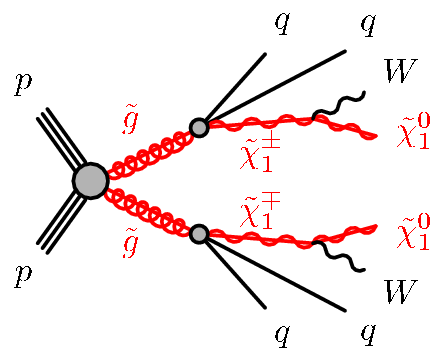
\includegraphics[width=.45\linewidth]{ATL-PHYS-PUB-2015-027/fig_01c}}
\subfloat[ ]{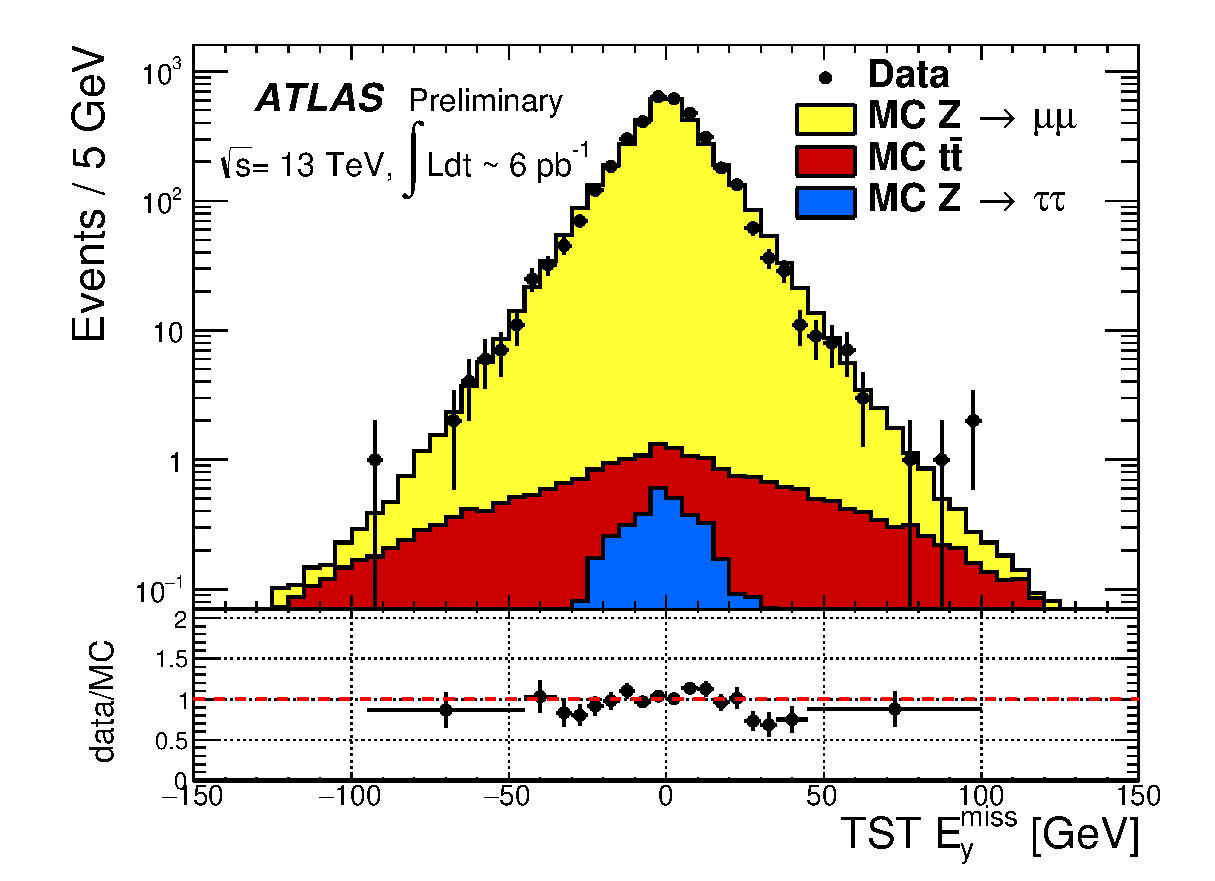
\includegraphics[width=.45\linewidth]{ATL-PHYS-PUB-2015-027/fig_01d}} \\
\subfloat[ ]{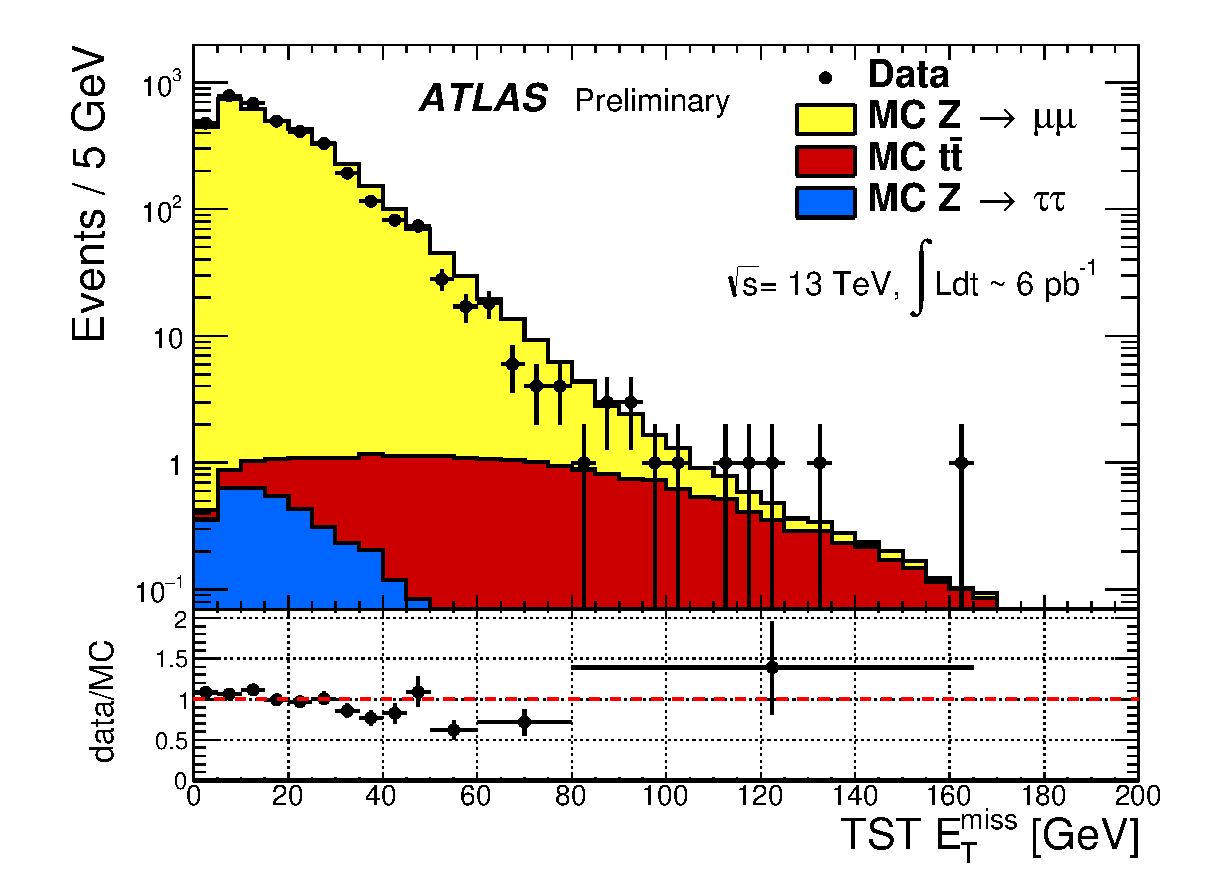
\includegraphics[width=.9\linewidth] {ATL-PHYS-PUB-2015-027/fig_01a}}
\end{figure}

\begin{figure}
\caption{Resolution of TST \met of early $\sqrt{s} = 13 \TeV$ data compared with simulation after the \Zmm selection described in Sec.\ref{subsubsec:met_event_selection}. The data sample consists of 6 \ipb.} \label{fig:tst_met_resolution_zmumu}
\subfloat[ ]{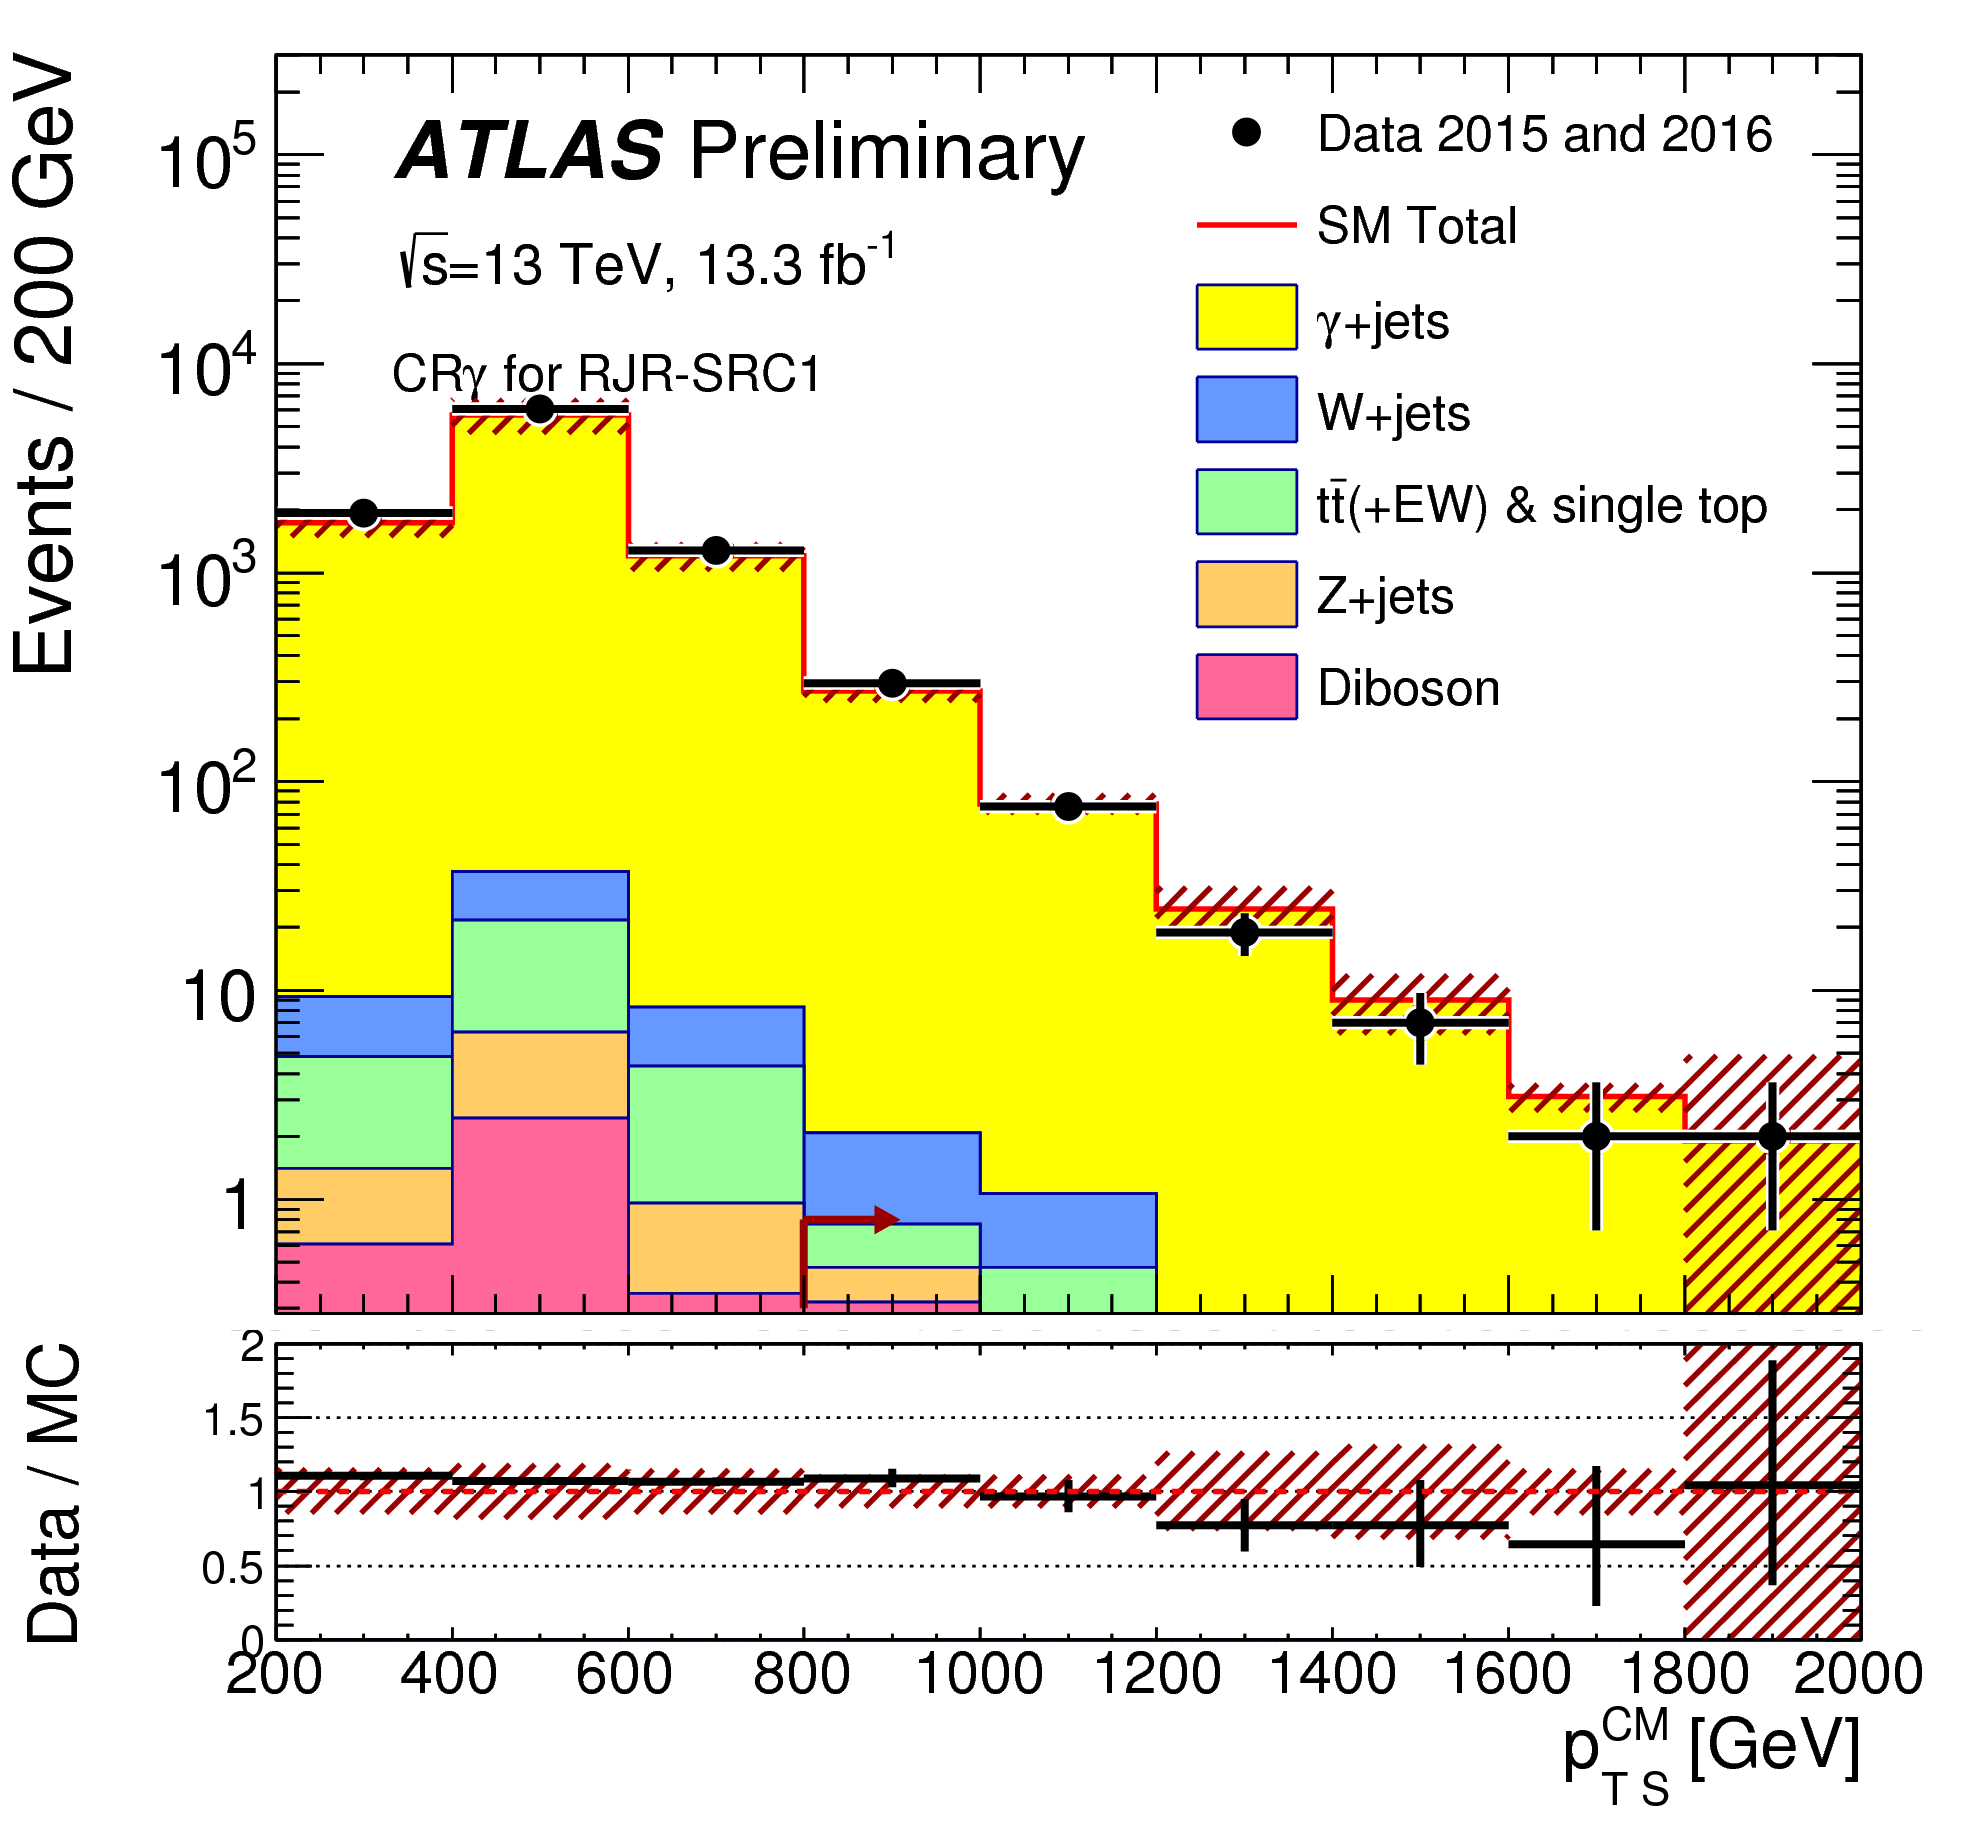
\includegraphics[width=.45\linewidth]{ATL-PHYS-PUB-2015-027/fig_04a}}
\subfloat[ ]{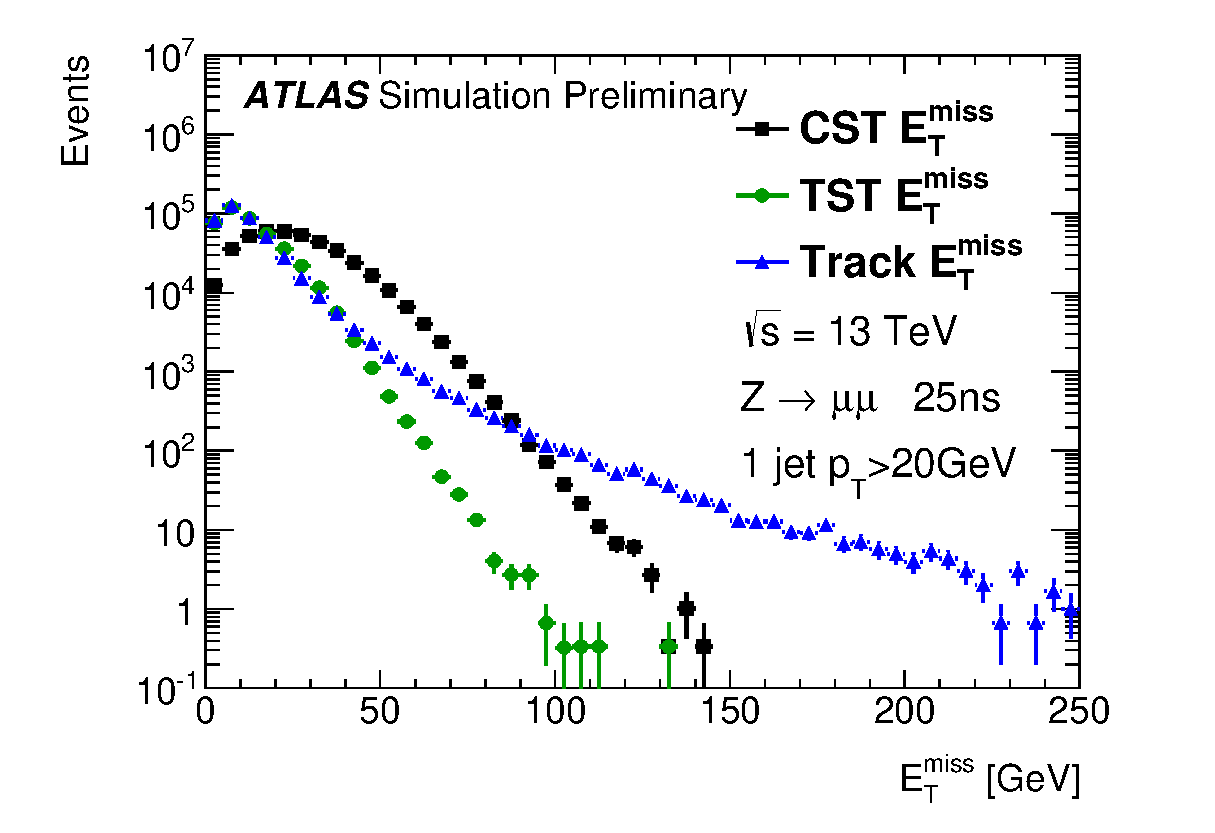
\includegraphics[width=.45\linewidth]{ATL-PHYS-PUB-2015-027/fig_04b}}
\end{figure}

\begin{figure}
\caption{Scale of TST \met of early $\sqrt{s} = 13 \TeV$ data compared with simulation after the \Zmm selection described in Sec.\ref{subsubsec:met_event_selection}. The data sample consists of 6 \ipb.} \label{fig:tst_met_scale_zmumu}
\subfloat[ ]{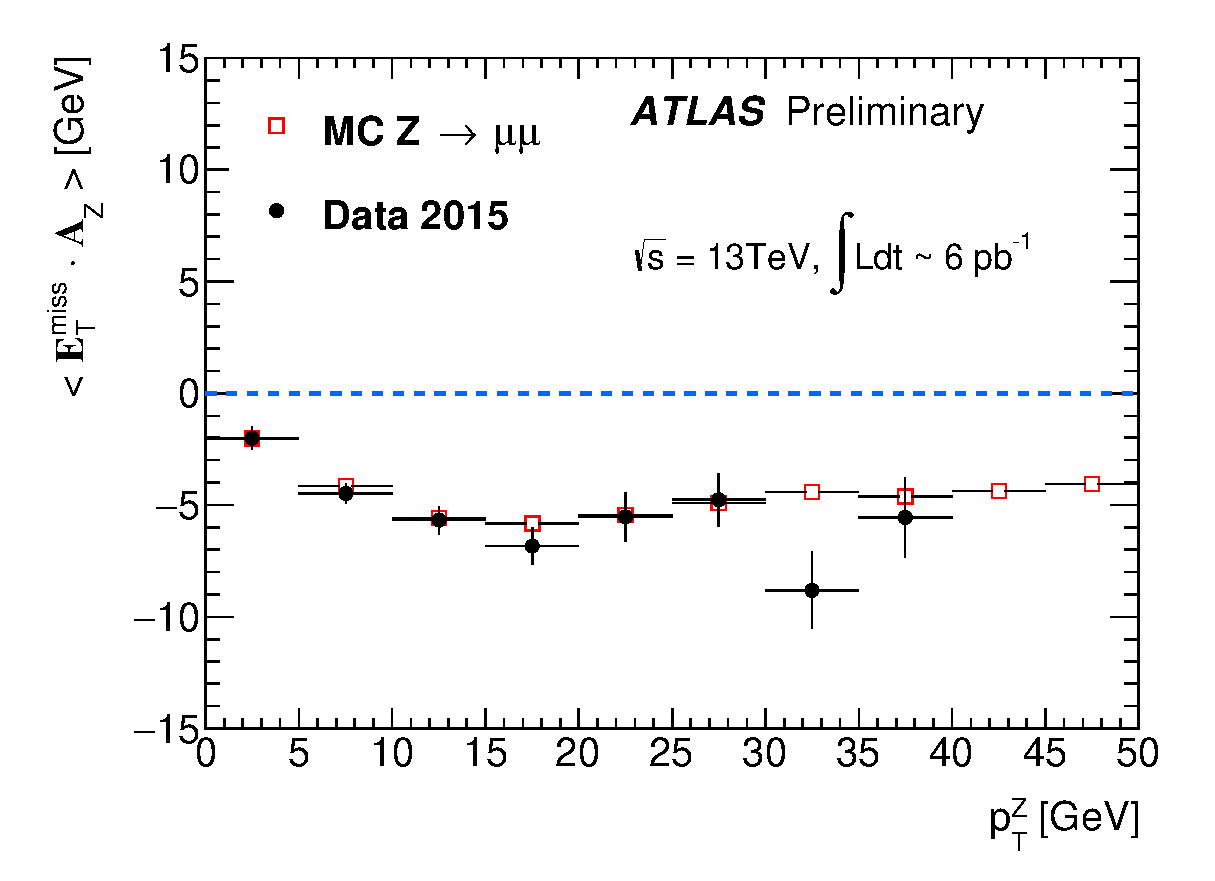
\includegraphics[width=.45\linewidth]{ATL-PHYS-PUB-2015-027/fig_05}}
\end{figure}


\subsubsection{Particle Flow Performance}

As described above, the resolution, scale, and linearity are the most important metrics to understand the performance of the different \met algorithms.
In this section, we present comparisons of the different algorithms, including particle flow, in simulation and using a data sample from 2015 of 80 \ipb.
In these plots, ``MET\_PFlow\_TST'' refers to charged PFlow \met, while the other algorithms are as described above.

Figures \ref{fig:mc_algs_met_resolution_zmumu,fig:mc_algs_met_scale_zmumu} show the resolution and scale in simulated \Zmm events.
The resolution curves follow the ``intuitive'' behavior discussed before.
Due to the high pileup in 2015 run conditions, the CST \met resolution is poor, and becomes even poorer with increasing pileup and event activity.
The ``regular'' PFlow \met shows reduces pileup and event activity dependence as compared to the CST.
As stated earlier, the \met from the PFlow algorithm can be seen as a hybrid of TST \met and CST \met.
The charged PFOs (\order 2/3) are pileup supressed, while the neutral PFOs (or topoclusters) are not.
Both charged PFlow and TST \met show only a small residual dependence on \npv and \sumET, since they have fully pileup supressed inputs through the track associations.

The scale plots are shown for $Z$+jets events and $Z$ events with no jets.
For the nonsuppressed CST, the scale continues to worsen with increasing \ptZ.
It is almost always the worst performing algorithm.
The standard PFlow algorithm performs the second worst in the region of high \ptZ, but is the best at low \ptZ.
The most exciting note in this plot is the improved scale of the charged PFlow \met compared to the TST \met.
Considering the resolution is essentially identical, the PFlow algorithm is better picking up the contributions from additional neutral particles.
In events with no jets, the soft term is essentially the only indication of the \met mismeasurement, since the muons will be well-measured.
In this case, the pileup effects cancel, on average, due to the U$(1)_\phi$ symmetry of the ATLAS detector, and CST performs rather well compared to the more complicated track-based algorithms.
The full PFlow algorithm performs best, since it provides a small amount of pileup suppression on the neutral components from CST.

The resolution and linearity are shown in simulated \Wen events in Figure \ref{fig:mc_algs_met_resolution_wenu,}.
The resolution in \Wen events shows a similar qualitative behavior to that shown in \Zmm events.
The CST \met has the worst performance, with charged PFlow \met performing best.
The surprise here is that the scale associated to TST \met in these events is best throughout the space parameterized by \mettrue, except for one bin at $40 \GeV < \mettrue < 50 \GeV$.
The scale in these events is best measured using a track-based soft term.

The resolution also investigated in real data passing the \Zmm selection described above.
A comparison of the \met between real data and simulation for each algorithm is presented in Figure \ref{fig:data_algs_met_zmumu}.
The resolution as a function of \sumET and \npv is shown in Figure \ref{fig:data_algs_met_resolution_zmumu} for this dataset.
Overall, this plot shows the same general features as the simulation dataset in terms of algorithm performance.
However, the performance of all algorithms seems to be significantly worse in data.
This is likely due to simplifications made in the simulation: soft interactions that cannot be simulated can have a significant effect on an event level variable such as the \met resolution.

\begin{figure}
\caption{Comparison of \met resolution and linearity using different \met algorithms with simulated \Wen events.} \label{fig:mc_algs_met_resolution_wenu}
\subfloat[ ]{\includegraphics[width=.45\linewidth]{HCW_plots/mc_algs_met_resolution_wenu}}
\subfloat[ ]{\includegraphics[width=.45\linewidth]{HCW_plots/mc_algs_met_linearity_wenu}}
\end{figure}

\begin{figure}
\caption{Comparison of \met resolution using different \met algorithms with simulated \Zmm events.} \label{fig:mc_algs_met_resolution_zmumu}
\subfloat[ ]{\includegraphics[width=.45\linewidth]{HCW_plots/resol_sumet_mc}}
\subfloat[ ]{\includegraphics[width=.45\linewidth]{HCW_plots/resol_npv_mc}}
\end{figure}

\begin{figure}
\caption{Comparison of \met scale using different \met algorithms with simulated \Zmm events.} \label{fig:mc_algs_met_scale_zmumu}
\subfloat[Inclusive in number of jets ]{\includegraphics[width=.45\linewidth]{HCW_plots/scale_ptz}}
\subfloat[Zero jet events ]{\includegraphics[width=.45\linewidth]            {HCW_plots/scale_ptz_no_jets}}
\end{figure}

\begin{figure}
\caption{Comparison of \met distributions using different \met algorithms with a data sample of 80 \ipb after the \Zmm selection described in Sec.\ref{subsubsec:met_event_selection}} \label{fig:data_algs_met_zmumu}
\subfloat[ ]{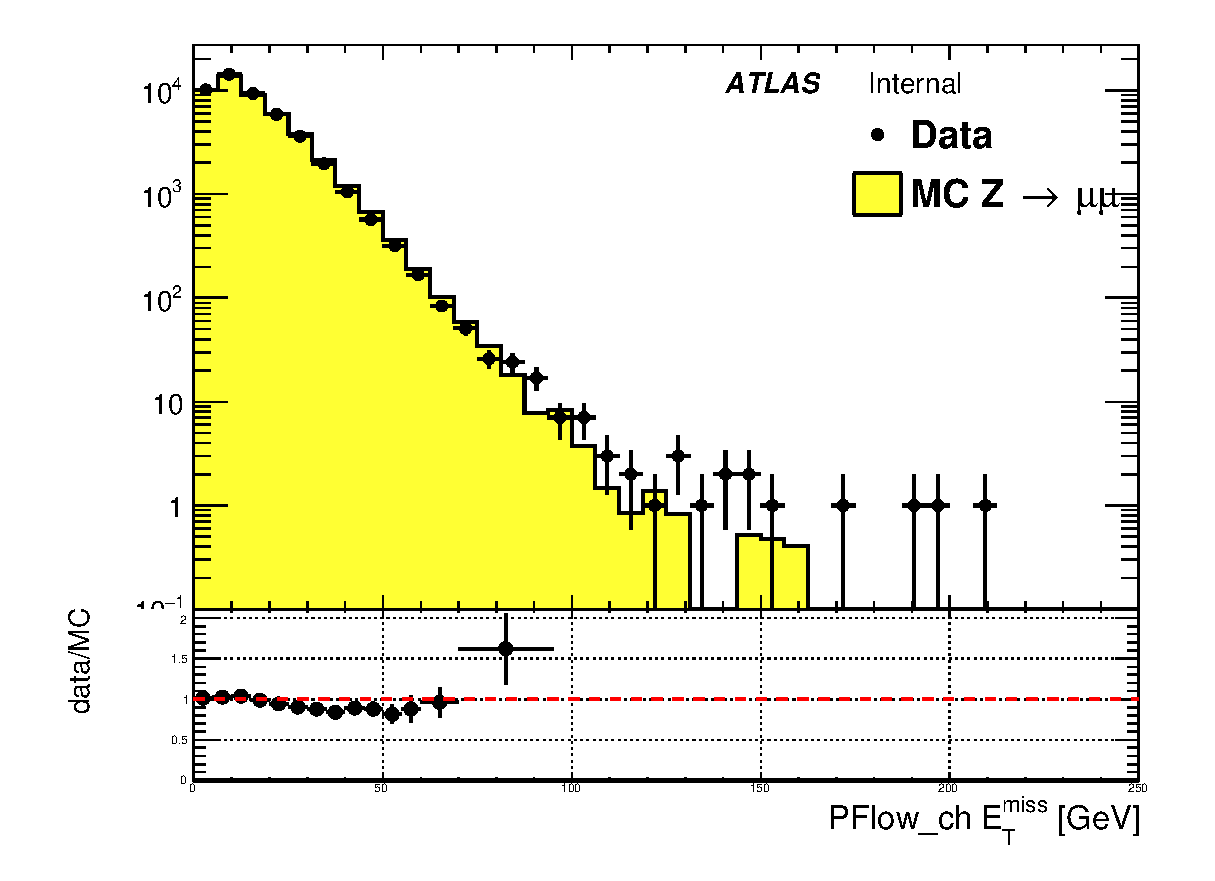
\includegraphics[width=.45\linewidth]{HCW_plots/MET_PFlow_ch_weight_zmumu}}
\subfloat[ ]{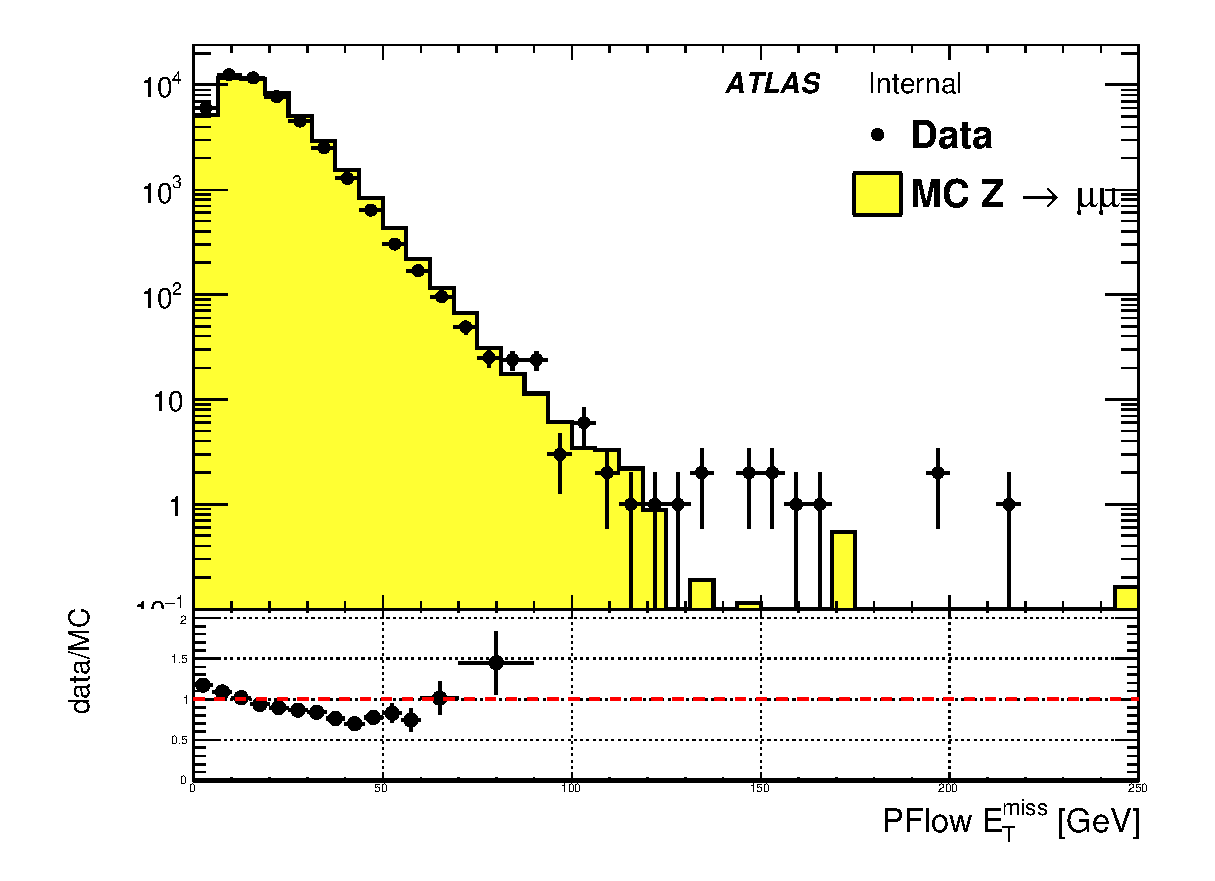
\includegraphics[width=.45\linewidth]{HCW_plots/MET_PFlow_weight_zmumu}} \\
\subfloat[ ]{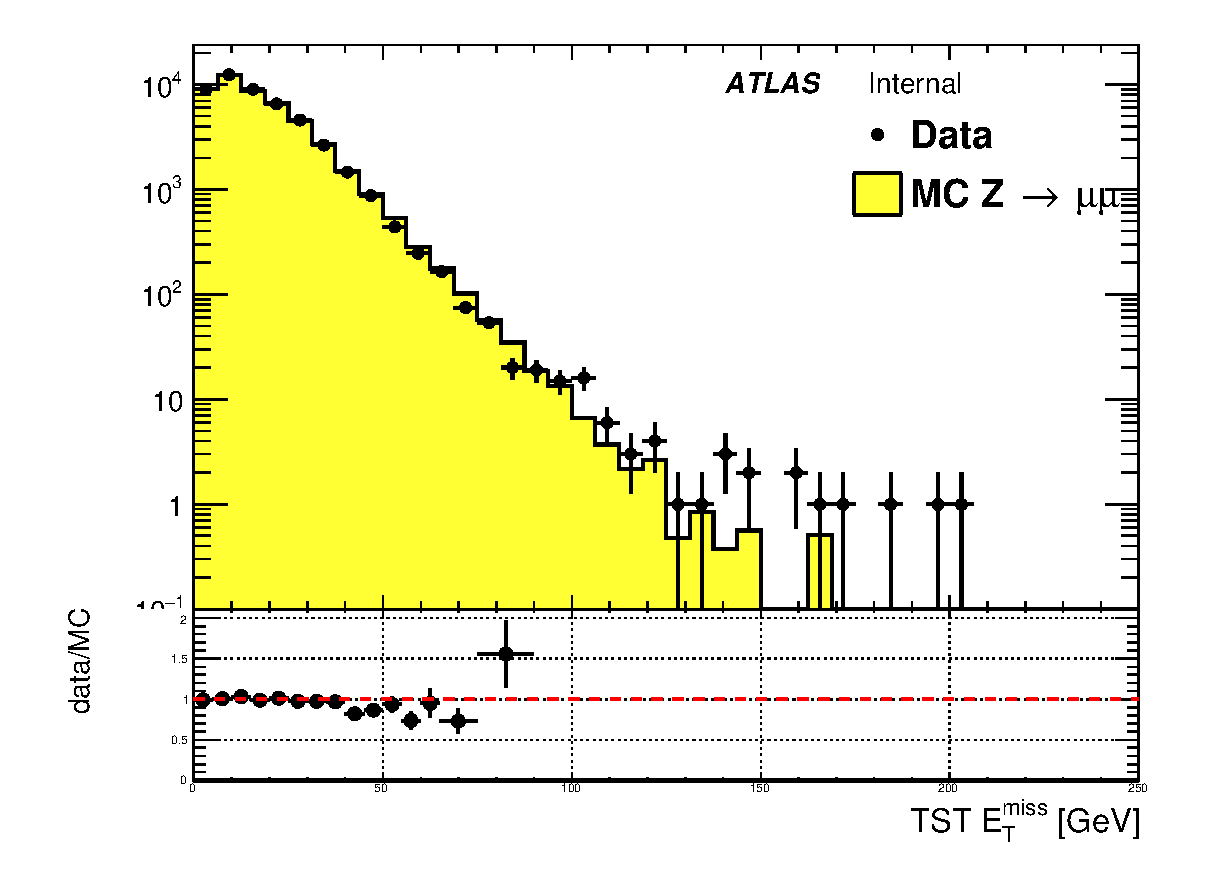
\includegraphics[width=.45\linewidth]{HCW_plots/MET_TST_weight_zmumu}}
\subfloat[ ]{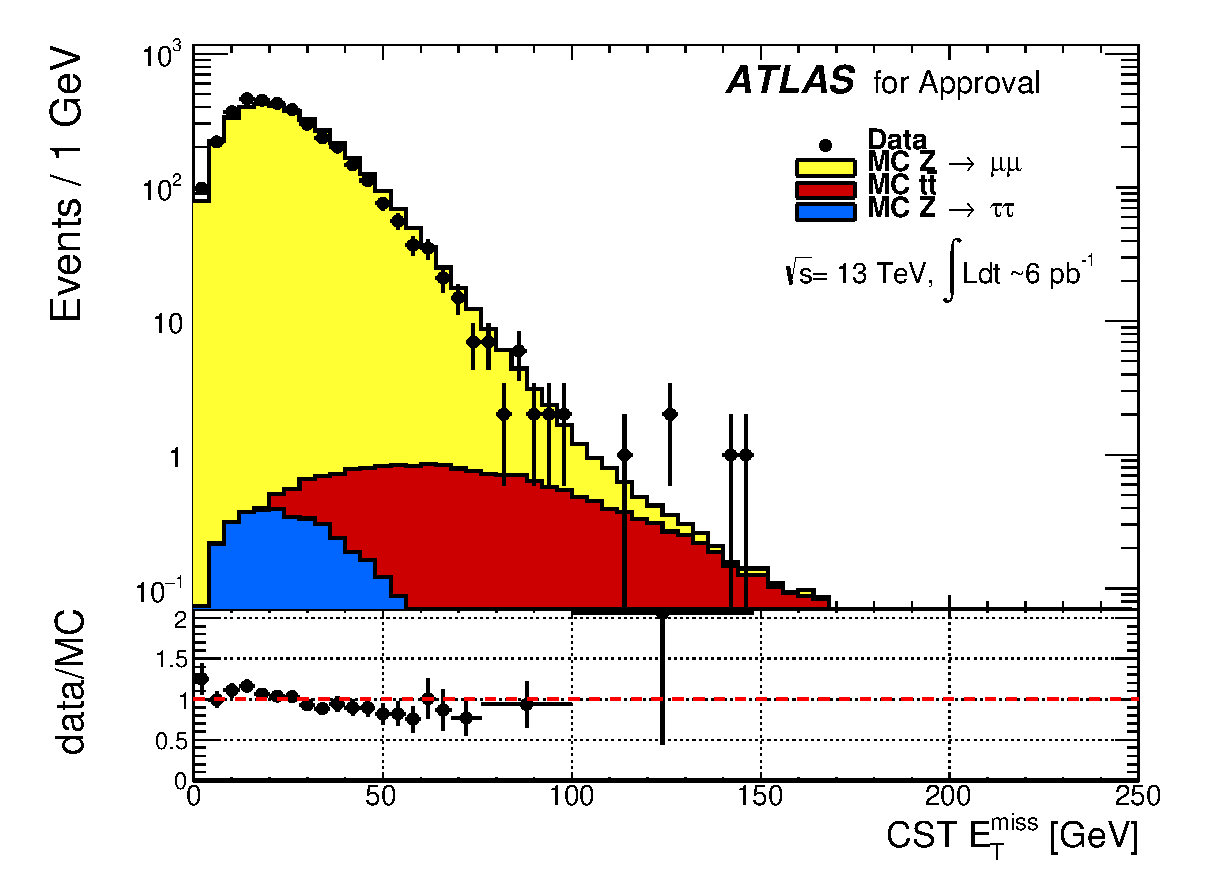
\includegraphics[width=.45\linewidth]{HCW_plots/MET_CST_weight_zmumu}}
\end{figure}


\begin{figure}
\caption{Comparison of \met resolution using different \met algorithms with a data sample of 80 \ipb after the \Zmm selection described in Sec.\ref{subsubsec:met_event_selection}} \label{fig:data_algs_met_resolution_zmumu}
\subfloat[ ]{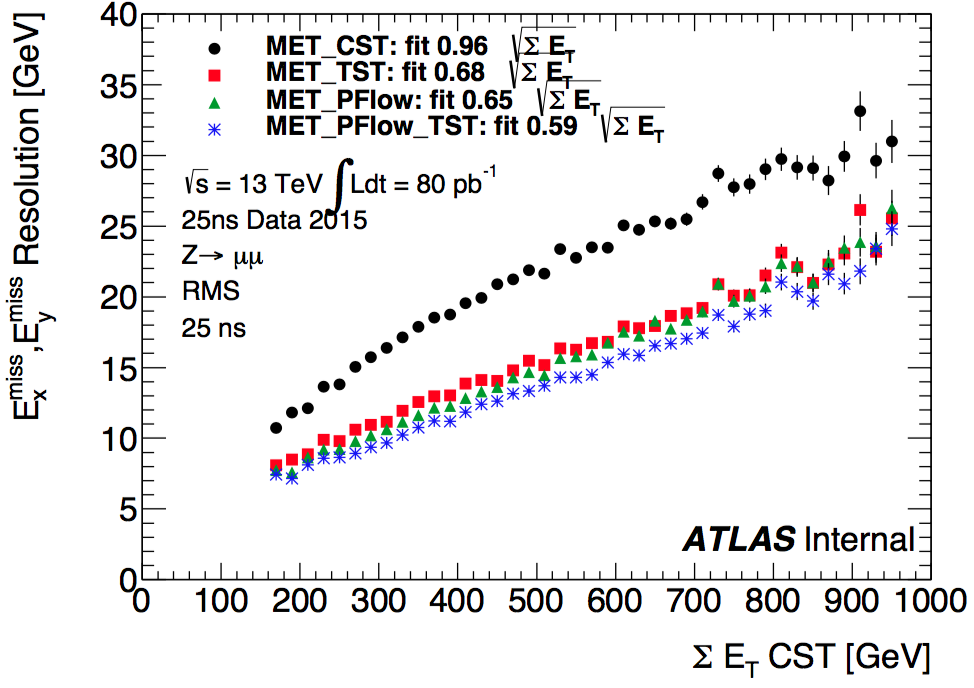
\includegraphics[width=.45\linewidth]{HCW_plots/resol_sumet}}
\subfloat[ ]{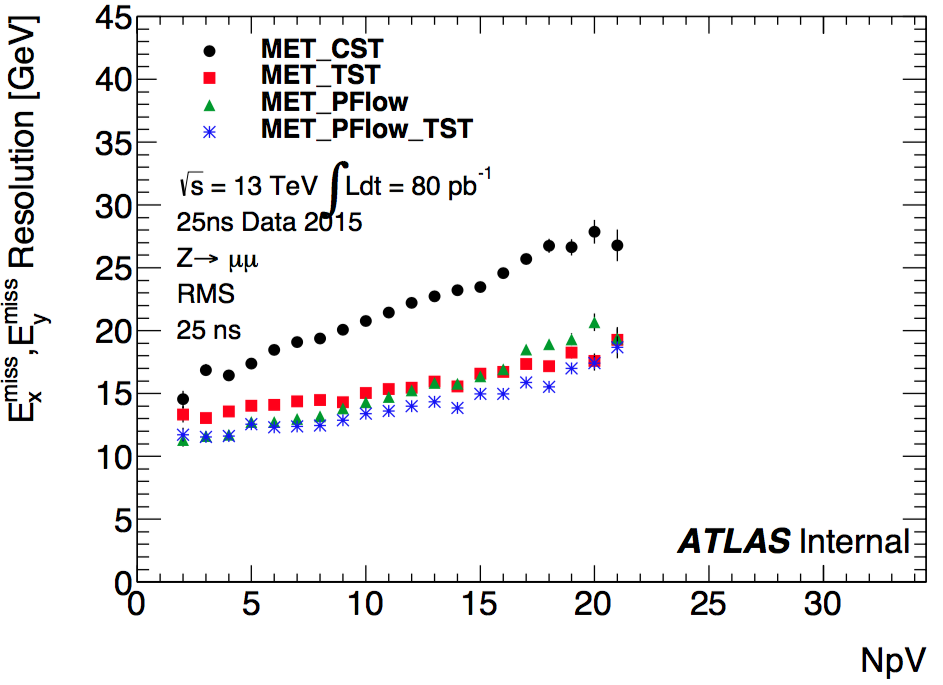
\includegraphics[width=.45\linewidth]{HCW_plots/resol_npv}}
\end{figure}
